\RCS$Revision: 450971 $
\RCS$HeadURL: svn+ssh://svn.cern.ch/reps/tdr2/papers/HIG-21-XXX/trunk/HIG-21-XXX.tex $
\RCS$Id: HIG-21-XXX.tex 450971 2018-03-14 11:21:02Z veelken $

\newlength\cmsFigWidth
\ifthenelse{\boolean{cms@external}}{\setlength\cmsFigWidth{0.85\columnwidth}}{\setlength\cmsFigWidth{0.4\textwidth}}
\ifthenelse{\boolean{cms@external}}{\providecommand{\cmsLeft}{top\xspace}}{\providecommand{\cmsLeft}{left\xspace}}
\ifthenelse{\boolean{cms@external}}{\providecommand{\cmsRight}{bottom\xspace}}{\providecommand{\cmsRight}{right\xspace}}

\newcommand{\metHT}{\ensuremath{H_{\mathrm{T}}^\text{miss}}\xspace}
\newcommand{\metLD}{\ensuremath{L_\mathrm{D}\xspace}}

\renewcommand{\mT}{\ensuremath{m_\mathrm{T}}}
\newcommand{\mTprime}{\ensuremath{m^{'}_\mathrm{T}}}

\renewcommand{\tauh}{\ensuremath{\Pgt_{\mathrm{h}}}\xspace}
\newcommand{\Plepton}{\ensuremath{\ell}}
\newcommand{\PLepton}{\ensuremath{\ell}}
\newcommand{\Ppizero}{\ensuremath{\Pgpz}}
\newcommand{\Pnu}{\ensuremath{\PGn}}
\newcommand{\Pnut}{\ensuremath{\PGn_{\Pgt}}}
\newcommand{\APnut}{\ensuremath{\PAGn_{\Pgt}}}
\renewcommand{\Pgg}{\ensuremath{\PGg}\xspace}
\newcommand{\Pggx}{\ensuremath{\PGg^{*}}\xspace}
\newcommand{\APnu}{\ensuremath{\overline{\Pnu}}\xspace}
\newcommand{\PHiggs}{\ensuremath{\PH}}
\newcommand{\Pbottom}{\ensuremath{\PQb}}
\newcommand{\Pcharm}{\ensuremath{\PQc}}
\newcommand{\APbottom}{\ensuremath{\PAQb}}
\newcommand{\Ptop}{\ensuremath{\PQt}}
\newcommand{\APtop}{\ensuremath{\PAQt}}
\renewcommand{\ttbar}{\ensuremath{\mathrm{\ptop\APtop}\text{+jets}}}
\newcommand{\Pquark}{\ensuremath{\PQq}}
\newcommand{\Pgluon}{\ensuremath{\Pg}}
\newcommand{\HH}{\ensuremath{\PHiggs\PHiggs}}
\newcommand{\ggHH}{\ensuremath{\Pgluon\Pgluon\PHiggs\PHiggs}}
\newcommand{\qqHH}{\ensuremath{\Pquark\Pquark\PHiggs\PHiggs}}
\newcommand{\mHH}{\ensuremath{m_{\PHiggs\PHiggs}}}
\newcommand{\V}{\ensuremath{\textrm{V}}}
\newcommand{\X}{\ensuremath{\textrm{X}}}

\renewcommand{\ss}{\ensuremath{\text{ss}}}
\newcommand{\jet}{\ensuremath{\mathrm{j}}}
\newcommand{\bjet}{\ensuremath{\mathrm{b}}}
\newcommand{\jj}{\ensuremath{\mathrm{jj}}}
\newcommand{\vis}{\ensuremath{\text{vis}}}

\newcommand{\fb}{\ensuremath{\text{fb}}}
\renewcommand{\fbinv}{\ensuremath{\fb^{-1}}}
\newcommand{\pb}{\ensuremath{\text{pb}}}
\renewcommand{\pbinv}{\ensuremath{\pb^{-1}}}

\newcommand{\kappal}{\ensuremath{\kappa_{\lambda}}}
\newcommand{\yt}{\ensuremath{\text{y}_{\Ptop}}}
\newcommand{\kappat}{\ensuremath{\kappa_{\Ptop}}}
\newcommand{\cW}{\ensuremath{\textrm{c}_{\PW}}}
\newcommand{\cWW}{\ensuremath{\textrm{c}_{\PW\PW}}}
\newcommand{\cZ}{\ensuremath{\textrm{c}_{\PZ}}}
\newcommand{\cZZ}{\ensuremath{\textrm{c}_{\PZ\PZ}}}
\newcommand{\kappaV}{\ensuremath{\kappa_{\V}}}
\newcommand{\kappaVV}{\ensuremath{\kappa_{\V\V}}}
\newcommand{\cg}{\ensuremath{\text{c}_{\Pgluon}}}
\newcommand{\cgg}{\ensuremath{\text{c}_{2\Pgluon}}}
\newcommand{\ctwo}{\ensuremath{\text{c}_{2}}}

\newlength\cmsTabSkip\setlength{\cmsTabSkip}{1ex}

\providecommand{\NA}{\ensuremath{\text{---}}}
\ifthenelse{\boolean{cms@external}}{\providecommand{\CL}{C.L.\xspace}}{\providecommand{\CL}{CL\xspace}}

\newcolumntype{C}[1]{>{\centering\let\newline\\\arraybackslash\hspace{0pt}}m{#1}}
\newcolumntype{L}[1]{>{\raggedright\let\newline\\\arraybackslash\hspace{0pt}}m{#1}}
\newcolumntype{R}[1]{>{\raggedleft\let\newline\\\arraybackslash\hspace{0pt}}m{#1}}

\cmsNoteHeader{HIG-21-XXX}
\title{Search for Higgs boson pair production in final states with electrons, muons, and hadronically decaying $\PGt$ leptons at $\sqrt{s} = 13$~\TeV}

\date{\today}

\abstract{
  The results of a search for Higgs ($\textrm{H}$) boson pair production in final states with electrons, muons, and hadronically decaying $\tau$ leptons is presented.
  The search is based on proton-proton collision data recorded by the CMS experiment at $\sqrt{s} = 13$~\TeV center-of-mass energy,
  corresponding to an integrated luminosity of $137.2$~fb$^{-1}$.
  Seven distinct final states, distinguished by the multiplicity of electrons and muons, collectively denoted by the symbol $\ell$,
  and of hadronically decaying $\tau$ leptons, denoted by the symbol $\tau_{\textrm{h}}$, are included in the analysis:
  $0\ell + 4\tauh$, $1\ell + 3\tau_{\textrm{h}}$, $2\ell$ of same-sign charge, $2\ell + 2\tau_{\textrm{h}}$, $3\ell$, $3\ell + 1\tau_{\textrm{h}}$, and $4\ell$.
  These final states target $\textrm{H}$ boson pair ($\textrm{HH}$) production in events in which the $\PHiggs$ boson pair decays into either $\textrm{WWWW}$, $\textrm{WW}\tau\tau$, or $\tau\tau\tau\tau$
  and the $\textrm{W}$ bosons and $\tau$ leptons subsequently decay either leptonically or hadronically.
  No evidence for a signal is found in the data and upper limits on the cross section for non-resonant as well as resonant $\textrm{HH}$ production are set.
  For the case of non-resonant $\textrm{HH}$ production with event kinematics equal to the kinematics expected in the Standard Model (SM),
  the observed (expected) upper limit on the cross section, at $95\%$ confidence level (CL), amounts to $XX$ ($XX$) times the rate expected in the SM.
  The results of the search are used to exclude regions in the plane of the $\textrm{H}$ boson coupling to the top quark and of the trilinear $\textrm{H}$ boson self-coupling.
  Assuming $\yt$ has the value expected in the SM, the trilinear $\PHiggs$ boson self-coupling is constrained to be within the interval $X.X < \lambda < X.X$.
  For resonant $\HH$ production, the observed (expected) limits on the $\HH$ production cross section range from $XX$ to $XX$ ($XX$ to $XX$)~\pb at $95\%$ CL, 
  depending on the mass of the resonance and on whether the resonance has spin $0$ or spin $2$.
}

\hypersetup{
pdfauthor={The CMS Collaboration},
pdftitle={Search for Higgs boson pair production in final states with electrons, muons, and hadronically decaying tau leptons at at sqrt(s) = 13 TeV},
pdfsubject={CMS},
pdfkeywords={CMS, physics}
}

\maketitle

\section{Introduction}
\label{sec:introduction}

In the eight years that have passed since the discovery of the Higgs ($\PHiggs$) boson~\cite{Higgs-Discovery_CMS,Higgs-Discovery_CMS_long,Higgs-Discovery_ATLAS},
many of its properties have already been measured with remarkable precision~\cite{HIG-14-042,HIG-15-002,ATLAS_SpinCP,HIG-14-018,HIG-16-041}. %% TODO: UPDATE! - AWB 2021.01.15
One important property which remains mostly unknown is the $\PHiggs$ boson self-coupling.
A precise measurement of this coupling is important, as this measurement allows us to reconstruct the Higgs potential,
and thus verify that the mechanism which breaks electroweak gauge symmetry is indeed the Higgs mechanism postulated by the Standard Model (SM).
The latter predicts the existence of trilinear as well as of quartic $\PHiggs$ boson self-couplings.
The quartic self-coupling, measured via triple $\PHiggs$ boson production, is not experimentally accessible at the LHC~\cite{de_Florian_2020},
even with the full luminosity of 3000~\fbinv which should be delivered after the high-luminosity LHC upgrade~\cite{HL-LHC-TDR}.
The trilinear self-coupling however is experimentally accessible, and can be determined using measurements of $\PHiggs$ boson pair ($\HH$) production.

In the SM, $\HH$ production proceeds via two different processes.

The leading order (LO) Feynman diagrams for the dominant ``gluon fusion'' ($\ggHH$) process are shown in the upper half of Fig.~\ref{fig:Feynman_ggHH_and_qqHH_sm}.
The left ``triangle'' diagram amplitude varies proportionally to the values of the $\PHiggs$ boson self-coupling ($\lambda$)
and the Yukawa coupling of the top quark $\yt$,
while the right ``box'' diagram amplitude is insensitive to $\lambda$ and varies as $\yt^{2}$.
The triangle and box diagrams interfere destructively, 
so the $\ggHH$ cross section exhibits a strong dependence on $\lambda$ and $\yt$.
We denote the ratios of $\lambda$ and $\yt$ to their SM expectations as $\kappal$ and $\kappat$, respectively.
By definition, these ``coupling strength modifiers'' have values $\kappal = 1$ and $\kappat = 1$ in the SM.
The SM cross section for $\HH$ production via $\ggHH$ has been computed to be $31.05^{+1.40}_{-1.98}$~\fb
at next-to-next-to-leading (NNLO) accuracy in quantum chromodynamics (QCD)~\cite{Grazzini:2018hh}.
Effects due to the finite mass of the top quark are included up to next-to-leading (NLO) accuracy in the calculation.

The LO Feynman diagrams for the subdominant ``vector-boson-fusion'' ($\qqHH$) process are shown in the lower half of Fig.~\ref{fig:Feynman_ggHH_and_qqHH_sm},
where ``$\VH$'' refers to either a $\PW$ or $\PZ$ boson.
Its SM cross section has been computed at next-to-next-to-next-to-leading order (N$^{3}$LO) in QCD
and amounts to $1.73 \pm 0.04\fb$~\cite{Dreyer:2018qbw}.
The interference between different $\qqHH$ diagrams causes the cross section to exhibit a strong dependence on the five SM couplings
$\lambda$, $\cW$, $\cWW$, $\cZ$, and $\cZZ$,
where the $\cW$ ($\cZ$) and $\cWW$ ($\cZZ$) denote, respectively, the trilinear and quartic $\PHiggs$ boson couplings to the $\PW$ ($\PZ$) boson.

Assuming the two couplings $\cW$ and $\cZ$ ($\cWW$ and $\cZZ$) to vary by the same amount with respect to their SM expectation, 
and denoting the corresponding coupling strength modifier by the symbol $\kappaV$ ($\kappaVV$), we have in total four free parameters
when analyzing $\HH$ production via the $\ggHH$ and $\qqHH$ processes: $\kappal$, $\kappat$, $\kappaV$, and $\kappaVV$.
Due to interference, deviations of these five coupling strength modifiers from unity not only affect the rate of $\HH$ production,
but also the distribution of the $\HH$ signal in kinematic observables.
The $\PHiggs$ boson pair mass distribution ($\mHH$) is particularly sensitive to variations in $\kappal$ and $\kappat$,
as these couplings affect the triangle and box diagram amplitudes differently.
As $\ggHH$ and $\qqHH$ production typically result in a broad $\mHH$ distribution,
they are referred to as ``non-resonant''.

\begin{figure}[h!]
\setlength{\unitlength}{1mm}
\begin{center}
\begin{picture}(170,73)(0,0)
\put(  2.5, 43.0){\mbox{\includegraphics*[height=30mm]{figures/ggHH_triangle.pdf}}}
\put( 90.5, 43.0){\mbox{\includegraphics*[height=30mm]{figures/ggHH_box.pdf}}}
\put( -1.0,  2.0){\mbox{\includegraphics*[height=30mm]{figures/qqHH_c2v.pdf}}}
\put( 58.0,  2.0){\mbox{\includegraphics*[height=30mm]{figures/qqHH_cv.pdf}}}
\put(117.0,  2.0){\mbox{\includegraphics*[height=30mm]{figures/qqHH_lambda.pdf}}}
\put( 39.0, 40.0){\small (a)}
\put(120.0, 40.0){\small (b)}
\put( 19.0,  0.0){\small (c)}
\put( 78.0,  0.0){\small (d)}
\put(137.0,  0.0){\small (e)}
\end{picture}
\end{center}
\caption{
  LO Feynman diagrams for SM non-resonant $\HH$ production via gluon fusion (a,b)
  and via vector-boson-fusion (c,d,e).
}
\label{fig:Feynman_ggHH_and_qqHH_sm}
\end{figure}

The presence of undiscovered particles, predicted by a variety of theories beyond the SM, may alter the $\HH$ production rate
as well as distributions in kinematic observables.
If they exist, such particles are expected to give rise to loop diagrams similar to the ones shown in Fig.~\ref{fig:Feynman_ggHH_eft}.
These loop contributions may enhance the $\HH$ production rate significantly,
as they occur at the same loop level as the triangle and box diagrams that govern $\HH$ production in the SM.
As none of these new particles have been discovered, their mass is presumed to be at the \TeV scale or higher,
well above the scale of the electroweak symmetry breaking.
Their high mass allows loop contributions of new particles to be approximated by contact interactions with the $\PHiggs$ boson
using an effective field theory (EFT) approach~\cite{Buchmuller:1985jz,Grzadkowski:2010es}.
We follow Ref.~\cite{Carvalho:2015ttv} and parametrize the contact interactions relevant for $\HH$ production by the couplings $\cg$, $\cgg$, and $\ctwo$,
referring to the interactions between two gluons and two $\PHiggs$ bosons, two gluons and one $\PHiggs$ boson, 
and two top quarks and two $\PHiggs$ bosons, respectively.
The corresponding Feynman diagrams for $\ggHH$ production are shown in Fig.~\ref{fig:Feynman_ggHH_eft}.
Although $\cg$, $\cgg$, and $\ctwo$ also alter the $\qqHH$ production rate,
our analysis of $\HH$ decays to multiple leptons
has little sensitivity to the $\qqHH$ process, due to the small signal yield, 
and we thus concentrate our analysis of $\HH$ production in the EFT approach on the $\ggHH$ process in this paper.

\begin{figure}[h!]
\setlength{\unitlength}{1mm}
\begin{center}
\begin{picture}(170,32)(0,0)
\put(  0.5, 2.0){\mbox{\includegraphics*[height=30mm]{figures/ggHH_cg.pdf}}}
\put( 53.0, 2.0){\mbox{\includegraphics*[height=30mm]{figures/ggHH_cgg.pdf}}}
\put(111.0, 2.0){\mbox{\includegraphics*[height=30mm]{figures/ggHH_c2.pdf}}}
\put( 16.0, 0.0){\small (a)}
\put( 73.5, 0.0){\small (b)}
\put(138.0, 0.0){\small (c)}
\end{picture}
\end{center}
\caption{
  LO Feynman diagrams for non-resonant $\HH$ production via gluon fusion in an EFT approach
  where contact interactions between (a) two gluons and two $\PHiggs$ bosons, (b) two gluons and one $\PHiggs$ boson, 
  and (c) two top quarks and two $\PHiggs$ bosons are parametrized by the three couplings $\cg$, $\cgg$, and $\ctwo$, respectively.
}
\label{fig:Feynman_ggHH_eft}
\end{figure}

An excess of $\HH$ signal events may also result from decays of new heavy particles into pairs of SM $\PHiggs$ bosons.
Various theories beyond the SM postulate such decays, in particular
two-Higgs doublet models~\cite{Craig:2013hca,Nhung:2013lpa},
composite Higgs models~\cite{Grober:2010yv,Contino:2010mh}, Higgs portal models~\cite{Englert:2011yb,No:2013wsa},
and models inspired by warped extra dimensions (WED)~\cite{Randall:1999ee}.  %% TODO: do we want more up-to-date references? -AWB 2020.01.16
In models inspired by WED, the new heavy particles may have spin $0$ (``radions'') or spin $2$ (``gravitons'')~\cite{Cheung:2000rw}.
In this paper, the width of heavy particle $\X$ is assumed to be negligible compared to the experimental resolution on $\mHH$, 
so that ``resonant'' $\X \to \HH$ production would create a peak in the reconstructed $\mHH$ distribution at the mass $m_{\X}$ of the resonance.
The Feynman diagram for this process is shown in Fig.~\ref{fig:Feynman_ggHH_resonant}.

\begin{figure}[h!]
\setlength{\unitlength}{1mm}
\begin{center}
\includegraphics*[height=36mm]{figures/ggHH_resonant.pdf}
\end{center}
\caption{
  LO Feynman diagrams for resonant $\HH$ production.
}
\label{fig:Feynman_ggHH_resonant}
\end{figure}

In this paper, we present the results of a search for non-resonant as well as resonant $\HH$ production
in final states with multiple electrons or muons ($\Plepton$) or hadronically decaying $\PGt$ leptons ($\tauh$).
The search is based on proton-proton ($\Pp\Pp$) collision data recorded by the CMS experiment at $\sqrt{s} = 13\TeV$ center-of-mass energy
and corresponding to an integrated luminosity of $137.2$~\fbinv.
Seven distinct final states or ``categories'', distinguished by the multiplicity of leptons and $\tauh$, are included in the analysis:
\twoLeptonssZeroTau, \threeLeptonZeroTau, \fourLeptonZeroTau, \threeLeptonOneTau, \twoLeptonTwoTau, \oneLeptonThreeTau, and \zeroLeptonFourTau,
where the symbol $\ss$ indicates that the two leptons have the same electric charge. 
These final states target $\HH$ signal events in which the $\PHiggs$ boson pair decays into either \WWWW, \WWtt, or \tttt,
and the $\PW$ bosons and $\PGt$ leptons subsequently decay either leptonically or hadronically.
Multi-variate (MVA) methods are used to distinguish the $\HH$ signal from backgrounds,
with dedicated MVAs for SM, EFT, and resonant hypotheses in each category.

Phenomenological studies of the prospects for discovering the $\HH$ signal in the \WWWW decay mode
are documented in Refs.~\cite{Baur:2002rb,Baur:2002qd,Li:2015yia,Adhikary:2017jtu,Ren:2017jbg}.
The ATLAS collaboration has published the results of a search for non-resonant as well as resonant $\HH$ production in the same decay mode in Ref.~\cite{Aaboud:2018ksn},
based on $36.1$~\fbinv of $\Pp\Pp$ collision data recorded at $\sqrt{s} = 13\TeV$.
These analyses focus on the $\twoLeptonssZeroTau$, $\threeLeptonZeroTau$, and $\fourLeptonZeroTau$ final states.
This paper presents the first search for $\HH$ pairs decaying to \WWtt and \tttt.
Searches for $\HH$ production in $\Pp\Pp$ collisions at $\sqrt{s} = 7$, $8$, and $13\TeV$
have previously been performed by the CMS and ATLAS collaborations in the decay modes 
$\Pbottom\Pbottom\PGg\PGg$~\cite{Aad:2014yja,Khachatryan:2016sey,Sirunyan:2018iwt,Aaboud:2018ftw}, 
$\Pbottom\Pbottom\Pbottom\Pbottom$~\cite{Khachatryan:2015yea,Aad:2015uka,Aaboud:2018knk,Sirunyan:2018zkk,Sirunyan:2018tki}, 
$\Pbottom\Pbottom\PGt\PGt$~\cite{Aad:2015xja,Sirunyan:2017tqo,Sirunyan:2017djm,Aaboud:2018sfw}, 
$\Pbottom\Pbottom\PW\PW$~\cite{Sirunyan:2017guj}, 
and $\PW\PW\PGg\PGg$~\cite{Aaboud:2018ewm}.
Limits on $\HH$ production obtained from a combination of these analyses have been published by the CMS and ATLAS collaboration 
in Refs.~\cite{Aad:2015xja,Sirunyan:2017tqo,Sirunyan:2018ayu}.

The paper is structured as follows.
A brief overview of the CMS detector is given in Section~\ref{sec:detector}.
In Section~\ref{sec:datasets}, we detail the datasets and simulation samples used.
The reconstruction of electrons, muons, $\tauh$, and jets,
along with various kinematic observables is detailed in Section~\ref{sec:eventReconstruction}.
This is followed by a description, in Section~\ref{sec:eventSelection}, of the event selection criteria applied in the seven search categories.
The multi-variate methods used to distinguish the $\HH$ signal from backgrounds are detailed in Section~\ref{sec:analysisStrategy}.
The estimation of these backgrounds is described in Section~\ref{sec:backgroundEstimation},
followed by a description of the relevant systematic uncertainties in Section~\ref{sec:systematicUncertainties}.
The statistical procedure used to extract the $\HH$ production rate and the results obtained by our analysis are presented in Section~\ref{sec:results}.
The paper concludes with a summary in Section~\ref{sec:summary}.

\section{The CMS detector}
\label{sec:detector}

The central feature of the CMS apparatus is a superconducting solenoid of $6$\unit{m} internal diameter, 
providing a magnetic field of $3.8$\unit{T}. 
Within the solenoid volume are a silicon pixel and strip tracker, 
a lead tungstate crystal electromagnetic calorimeter (ECAL), 
and a brass and scintillator hadron calorimeter (HCAL), 
each composed of a barrel and two endcap sections.
The silicon tracker measures charged particles within the pseudorapidity range $\abs{\eta} < 2.5$. 
The ECAL is a fine-grained hermetic calorimeter with quasi-projective geometry,
and is segmented into the barrel region of $\abs{\eta} < 1.48$ and in two endcaps that extend up to $\abs{\eta} < 3.0$.
The HCAL barrel and endcaps similarly cover the region $\abs{\eta} < 3.0$.
Forward calorimeters extend the coverage up to $\abs{\eta} < 5.0$.
Muons are detected within the range $\abs{\eta} < 2.4$ 
by gas-ionization detectors embedded in the steel flux-return yoke outside the solenoid.
Events of interest are selected using a two-tiered trigger system. 
The first level, composed of custom hardware processors, uses information from the calorimeters and muon detectors 
to select events at a rate of around $100$\unit{kHz} within a fixed latency of about $4$\mus~\cite{Sirunyan:2020zal}. 
The second level, known as the high-level trigger, 
consists of a farm of processors running a version of the full event reconstruction software optimized for fast processing, 
and reduces the event rate to around $1$\unit{kHz} before data storage~\cite{Khachatryan:2016bia}. 
A more detailed description of the CMS detector, 
together with a definition of the coordinate system used and the relevant kinematic variables, can be found in Ref.~\cite{Chatrchyan:2008zzk}. 

\section{Data samples and Monte Carlo simulation}
\label{sec:datasets}

The data analyzed represent a total of 137.2~\fbinv of proton-proton collisions
collected by the CMS detector in Run~2, and certified to have all detector components
working properly: 35.9~\fbinv in 2016, 41.5~\fbinv in 2017, and 59.7~\fbinv in 2018.
The two-tier CMS ``trigger'' system selects one event of interest out of every thirty
thousand collision events to save for closer examination, based on the presence of
specific combinations of reconstructed objects.~\cite{CMS_trigger}  This analysis
uses triggers requiring one or more electrons, muons, or hadronically-decaying \Pgt
leptons to be associated with the leading primary vertex. The exact triggers and their
thresholds varied slightly from year to year, due to changing luminosity and detector
conditions, as well as improvements to the trigger algorithms.  The trigger \pt and
$\eta$ requirements for each year are shown in Table~\ref{tab:HH_triggers}.  All
triggers included identification and isolation requirements on the leptons as well.

\begin{table}[!h]
\begin{center}

%% \begin{tabular}{|l|c|c|c|}
%% \hline
%% Trigger              & Electron selection  & Muon selection & Tau selection \\
%% \hline
%% Single electron      & $\pt > 25$~GeV (and $|\eta| < 2.1$) or $27$~GeV / $32 -- 35$~GeV / $32$~GeV (2016/17/18) &  &  \\
%% Single muon          &  & $\pt > 22 -- 24 / 24 -- 27 / 24$~GeV (2016/17/18) &  \\ 
%% Double electron      & $\pt > 23$ and $12$~GeV &  &  \\
%% Electron + muon      & $\pt > 23$ or $8 / 12 / 12$~GeV (2016/17/18) & $\pt > 8$ or $23$~GeV &  \\
%% Double muon          &  & $\pt > 17$ and $8$~GeV &  \\
%% Electron + tau       & $\pt > 24$~GeV and $|\eta| < 2.1$ &  & $\pt > 20 -- 30 / 30 / 30$~GeV and $|\eta| < 2.1$ (2016/17/18) \\
%% Muon + tau           &  & $\pt > 19 / 20 / 20$~GeV and $|\eta| < 2.1$ (2016/17/18) & $\pt > 20 / 27 / 27$~GeV and $|\eta| < 2.1$ (2016/17/18) \\
%% Double tau           &  &  & Both $\pt > 35 -- 40$~GeV $|\eta| < 2.1$  \\
%% Triple electron      & $\pt > 16, 12,$ and $8$~GeV &  &  \\
%% Two electron + muon  & Both $\pt > 12$~GeV & $\pt > 8$~GeV &  \\
%% Two muon + electron  & $\pt > 9$~GeV & Both $\pt > 9$~GeV &  \\
%% Triple muon          &  & $\pt > 12, 10,$ and $5$~GeV &  \\
\hline

\begin{tabular}{|l|l|}
\hline
Trigger          & Object selection (electron $e$, muon $\mu$, and hadronic tau \tauh) \\
\hline
Single $e$       & $\pt(e) > 27 / 32 - 35 / 32$~GeV (2016/17/18) \\
Single $\mu$     & $\pt(\mu) > 22 - 24 / 24 - 27 / 24$~GeV (2016/17/18) \\ 
Double $e$       & $\pt(e) > 23, 12$~GeV \\
$e$ + $\mu$      & $\pt(e) > 23$~GeV, $\pt(\mu) > 8$~GeV \\
$\mu$ + $e$      & $\pt(\mu) > 23$~GeV, $\pt(e) > 8 / 12 / 12$~GeV (2016/17/18) \\
Double $\mu$     & $\pt(\mu) > 17, 8$~GeV \\
$e$ + \tauh      & $\pt(e) > 24$~GeV, $\pt(\tauh) > 20 - 30 / 30 / 30$~GeV, $|\eta(e, \tauh)| < 2.1$ (2016/17/18) \\
$\mu$ + \tauh    & $\pt(\mu) > 19 / 20 / 20$~GeV, $\pt(\tauh) > 20 / 27 / 27$~GeV, $|\eta(\mu, \tauh)| < 2.1$ (2016/17/18) \\
Double \tauh     & $\pt(\tauh) > 35 - 40, 35 - 40$~GeV, $|\eta(\tauh)| < 2.1$  \\
Triple $e$       & $\pt(e) > 16, 12, 8$~GeV \\
Two $e$ + $\mu$  & $\pt(e) > 12, 12$~GeV, $\pt(\mu) > 8$~GeV \\
Two $\mu$ + $e$  & $\pt(\mu) > 9, 9$~GeV, $\pt(e) > 9$~GeV \\
Triple $\mu$     & $\pt(\mu) > 12, 10, 5$~GeV \\
\hline

\end{tabular}
\end{center}
\caption{
  Selection requirements on \pt and $\eta$ for lepton-triggered events used in this analysis.  All
  leptons were additionally required to pass identification, isolation, and vertexing requirements.
}
\label{tab:HH_triggers}
\end{table}

%% TODO: how were events "cross-cleaned" between datasets? (AWB 11.01.21)

Monte Carlo (MC) simulated samples were used to model HH signal events, and a wide range
of SM background processes which can produce multiple leptons.  Background MC samples
include those producing a single W or Z boson, two bosons (WW, WZ, ZZ, W$\gamma$, and Z$\gamma$),
three bosons (WWW, WWZ, WZZ, ZZZ, and WZ$\gamma$), a single Higgs boson (via gluon fusion,
vector boson fusion, or associated production with a W or Z boson), a single top quark,
a top anti-top quark pair (\tops), and top quarks associated with one or more bosons (\ttW,
\ttZ, \ttH, \tHq, and \topHW).  Most samples, including the dominant irreducible WZ and ZZ
backgrounds, were generated at next-to-leading-order (NLO) and scaled to cross sections
computed at next-to-next-to-leading-order (NNLO).

A variety of HH signal samples were generated, including Higgs pairs produced via gluon
fusion (gg) and vector boson fusion (VBF) where both Higgs decay to either WW, ZZ, or \Pgt\Pgt.
Non-resonant di-Higgs MC samples include SM production, ``box-only'' di-Higgs events with
the trilinear Higgs self-coupling ($\kappa_{\lambda}$) set to 0, and 12 benchmark models
from effective field theory (EFT).  These benchmarks represent different combinations of
$\kappa_{\lambda}$, $\kappa_{t}$, $c_{2}$, $c_{g}$, and $c_{2g}$ values which correspond
to regions of similar LO kinematics, described in~\cite{Xandra:2016hhBM}.  The parameter
values are shown in Table~\ref{tab:HH_benchmarks}.  The EFT benchmark samples were
generated at LO but reweighted using the $aMC@NLO$ model described
in~\cite{Frixione:2011NLOQCD,Alwall:2014dcshh}.

\begin{table}[!h]
\begin{center}
\begin{tabular}{|l|c|c|c|c|c|} \hline
Benchmark & $\kappa_{\lambda}$  & $\kappa_{t}$ & $c_{2}$ & $c_{g}$ &  $c_{2g}$ \\
\hline
1         & 7.5                 & 1.0          & -1.0    & 0.0     & 0.0 \\
2         & 1.0                 & 1.0          &  0.5    & -0.8    & 0.6 \\
3         & 1.0                 & 1.0          & -1.5    & 0.0     & -0.8 \\
4         & -3.5                & 1.5          & -3.0    & 0.0     & 0.0 \\
5         & 1.0                 & 1.0          & 0.0     & 0.8     & -1.0 \\
6         & 2.4                 & 1.0          & 0.0     & 0.2     & -0.2 \\
7         & 5.0                 & 1.0          & 0.0     & 0.2     & -0.2 \\
8         & 15.0                & 1.0          & 0.0     & -1.0    & 1.0 \\
9         & 1.0                 & 1.0          & 1.0     & -0.6    & 0.6 \\
10         & 10.0                & 1.5          & -1.0    & 0.0     & 0.0 \\
11        & 2.4                 & 1.0          & 0.0     & 1.0     & -1.0 \\
12        & 15.0                & 1.0          & 1.0     & 0.0     & 0.0 \\
\hline
SM        & 1.0                 & 1.0          & 0.0     & 0.0     & 0.0 \\
box       & 0.0                 & 1.0          & 0.0     & 0.0     & 0.0 \\
\hline
\end{tabular}
\end{center}
\caption{
  Parameter values for $\kappa_{\lambda}$, $\kappa_{t}$, $c_{2}$, $c_{g}$, and
  $c_{2g}$ in MC samples modeling twelve BSM EFT benchmark scenarios, plus SM
  and ``box-only'' HH production.
}
\label{tab:HH_benchmarks}
\end{table}

Resonant di-Higgs production was simulated at LO for both spin-0 (radion) and spin-2 (graviton)
scenarios with invariant masses of 250, 260, 270, 280, 300, 320, 350, 400, 450, 500, 550, 600,
650, 700, 750, 800, 850, 900, and 1000~TeV.

All MC samples were generated using $\textsc{MadGraph5\_aMCatNLO}$~\cite{MadGraph5_aMCatNLO} or
$\textsc{POWHEG}$ $v2$~\cite{POWHEG1,POWHEG2,POWHEG3}, with parton shower, hadronization
processes, and \Pgt lepton decays modeled by
$\textsc{PYTHIA}$~\cite{PYTHIA_CUETP8M1tune_CMS,PYTHIA_CUETP8M2tune_CMS,CP5tune_CMS,PYTHIA_MonashTune}.
The CMS apparatus was modeled in detail using $\textsc{geant4}$~\cite{geant4}, and simulated events
were reconstructed identically to data.  Additional collisions were generated with $\textsc{PYTHIA}$ and
overlaid on all MC events, with weights used to match the collision multiplicity distribution to data.

\section{Event reconstruction}
\label{sec:eventReconstruction}

The CMS particle-flow (PF) algorithm~\cite{Sirunyan:2017ulk} reconstructs each individual particle in an event,
using an optimized combination of information from the various elements of the CMS detector.
The particles are subsequently classified into five mutually exclusive categories: 
electrons, muons, photons, and charged and neutral hadrons.
These particles are then combined to reconstruct hadronic $\PGt$ decays, jets, and the missing transverse momentum in the event.

Electrons are reconstructed within the geometric acceptance of the tracking detectors ($\abs{\eta} < 2.5$)
by combining information from the tracker and the ECAL~\cite{Khachatryan:2015hwa}.
They are initially identified using an MVA which distinguishes real electrons from hadrons, %% ~\cite{TODO: CMS EGamma}
along with loose requirements on track association with the collision vertex, and isolation from hadronic activity.
Electrons passing this intial selection are referred to as ``loose''.
In this analysis, events with leptons originating from hadron decay (``non-prompt''), or with
hadrons mis-identified as electrons (``fake''), consititute the largest source of background.
This motivates the use of an additional MVA, trained to select ``prompt'' electrons
from $\PW$, $\PZ$, and $\PGt$ decay, and reject fake or non-prompt electrons.
This MVA was previously used for measurements of $\ttH$ production in events with multiple leptons~\cite{Sirunyan:2020icl}.
It combines observables comparing measurements of the electron energy and direction in the tracker and the ECAL,
the compactness of the electron cluster, the bremsstrahlung emitted along the electron trajectory,
and the isolation of the electron with respect to other particles.
Electrons passing loose and tight thresholds of the MVA output are referred to as ``fakeable'' and ``tight'' electrons, respectively.
Only ``tight'' electrons are used to reconstruct signal candidate events, while data events with ``fakeable'' electrons which fail
the ``tight'' selection are used to estimate the contribution of fake and non-prompt electron backgrounds to the signal region.
The MVA selection thresholds in this analysis are lower than those in Ref.~\cite{Sirunyan:2020icl}, in order to increase
the efficiency for low-$\pt$ electrons which frequently appear in $\HH$ decays.
Electrons from photon conversions are suppressed by requiring that the track is missing no hits
in the innermost layers of the silicon tracker, and is not matched to a reconstructed conversion vertex.
In the \twoLeptonssZeroTau category, further electron selection criteria are applied,
requiring consistency among three independent measurements of the electron charge~\cite{Khachatryan:2015hwa}.

Muons are reconstructed by extrapolating tracks in the silicon tracker to hits in the gas-ionization
detectors embedded in the steel flux-return yoke outside the solenoid~\cite{Sirunyan:2018}.
To pass the initial ``loose'' identification requirement, muons must satisfy criteria related to
isolation and track proximity to the primary vertex, as well as track quality observables and
matching between the tracker and muon chambers. %% ~\cite{TODO: CMS Muon POG}
Additional requirements on the prompt vs.\ non-prompt muon identification MVA from Ref.~\cite{Sirunyan:2020icl} allow
us to select ``tight'' muons for signal candidate events, and ``fakeable'' muons for non-prompt background estimation.
Inputs to this MVA include energy deposits close to the muon in the ECAL and HCAL,
the hits and track segments reconstructed in the gas-ionization detectors located outside the solenoid,
the quality of the spatial matching between the track segments reconstructed in the silicon tracker and in the gas-ionization detectors,
and the isolation of the muon with respect to other particles.
Again, lower MVA selection thresholds compared to Ref.~\cite{Sirunyan:2020icl} bring higher efficiency for the $\HH$ signal.
In the \twoLeptonssZeroTau channel, the uncertainty in the curvature of the muon track is required to be less than $20\%$
to ensure a high-quality charge measurement.

Hadronic decays of $\PGt$ leptons are identified using the ``hadrons-plus-strips'' (HPS) algorithm~\cite{Sirunyan:2018pgf}.
This algorithm classifies individual hadronic decay modes of the $\PGt$ lepton
by combining charged hadrons from the PF reconstruction with neutral pions.
The latter are reconstructed by clustering electrons and photons into rectangular strips,
which are narrow in $\eta$ but wide in the $\phi$ direction.
The spread in $\phi$ accounts for photons originating from neutral pion decays
which convert into electron-positron pairs when traversing the silicon tracker.
These electrons and positrons are bent in opposite directions in $\phi$ by the magnetic field,
and may further emit bremsstrahlung photons while traversing the tracker.
The decay modes considered in this analysis are
$\PGt^{-} \to \Ph^{-}\Pnut$, $\PGt^{-} \to \Ph^{-}\Ppizero\Pnut$, $\PGt^{-} \to \Ph^{-}\Ppizero\Ppizero\Pnut$, 
$\PGt^{-} \to \Ph^{-}\Ph^{+}\Ph^{-}\Pnut$, and $\PGt^{-} \to \Ph^{-}\Ph^{+}\Ph^{-}\Ppizero\Pnut$
(plus the charge-conjugate decays),
where $\Ph^{-}$ and $\Ph^{+}$ denote charged pions or kaons.
The``DeepTau'' algorithm~\cite{CMS-DP-2019-033} identifies $\tauh$ objects
using a convolutional artificial neural network (ANN)~\cite{lecun1989}
with $42$ high-level observables as input, plus low-level information obtained from the silicon tracker, the electromagnetic and hadronic calorimeters, and the muon detectors.
The former comprise the $\pt$, $\eta$, $\phi$, and mass of the $\tauh$ candidate, the reconstructed $\tauh$ decay mode,
its isolation with respect to charged and neutral particles,
and the estimated distance that the $\Pgt$ lepton traverses between its production and decay.
The low-level information quantifies the particle activity within two $\eta \times \phi$ grids, centered on the direction of the $\tauh$ candidate:
an ``inner'' grid of size $0.2 \times 0.2$, filled with $0.02 \times 0.02$ cells,
and an ``outer'' grid of size $0.5 \times 0.5$ (partially overlapping with the inner grid), with $0.05 \times 0.05$ cells.
The $\tauh$ considered in this analysis are required to satisfy the conditions $\pt > 20\GeV$ and $\abs{\eta} < 2.3$,
and to pass a loose or tight selection on the output of the ANN, designating ``fakeable'' and ``tight'' $\tauh$, respectively.
Additional discriminants are used to separate $\tauh$ from electrons and muons.

Jets ($\jet$) are reconstructed with the infrared and collinear safe anti-\kt algorithm~\cite{Cacciari:2008gp, Cacciari:2011ma},
using PF reconstructed particles as input,
and serve to identify $\PHiggs \to \PW\PW \to \jet\jet\Plepton\Pnu$ decays in this analysis.
Jets reconstructed with distance parameters of $0.4$ (``AK4'') and $0.8$ (``AK8'') are both used:
two AK4 jets to reconstruct the two quarks from low-$\pt$ $\PW$ decays, or a single AK8 jet to reconstruct high-$\pt$
$\PW$ decays, where the quarks are collimated.
As the leptons produced in $\PHiggs \to \PW\PW$ decays with boosted $\PW$ bosons tend to be close to the jets,
leptons are removed from the AK8 jet reconstruction.
%% %% I don't think we need to describe the full jet calibration and validation procedure.
%% %% Jets are our least-important object, and we don't go into nearly this much detail for electrons or muons. - AWB 11.02.2021
%% The momentum of AK4 and AK8 jets is determined as the vectorial sum of all particle momenta in the jet,
%% and is found from simulation to be, on average, within $5$ to $10\%$ of the true momentum over the whole $\pt$ spectrum and detector acceptance.
%% Additional $\Pp\Pp$ interactions within the same or nearby bunch crossings (pileup) can contribute additional tracks and calorimetric energy depositions to the jet momentum.
%% To mitigate this effect, charged particles identified to be originating from pileup vertices are discarded and an offset correction is applied to correct for remaining contributions.
%% Jet energy corrections are derived from simulation to bring the measured response of jets to that of particle level jets on average.
%% In situ measurements of the momentum balance in dijet, $\text{photon} + \text{jet}$, $\PZ + \text{jet}$, and multijet events
%% are used to account for any residual differences in the jet energy scale between data and simulation~\cite{Khachatryan:2016kdb}.
After correcting for energy deposits from additional $\Pp\Pp$ interactions (pileup) and applying energy calibration,
the jet energy resolution amounts to $15$--$20\%$ at $30\GeV$, $10\%$ at $100\GeV$, and $5\%$ at $1\TeV$~\cite{Khachatryan:2016kdb}.
%% Additional selection criteria are applied to each jet to remove jets potentially dominated by anomalous contributions from various subdetector components or reconstruction failures.
This analysis considers jets reconstructed in the region $\abs{\eta} < 2.4$
with $\pt > 25\GeV$ (for AK4 jets) or $\pt > 170\GeV$ (for AK8 jets).
Additional criteria are applied to AK8 jets to specifically select those from boosted hadronic $\PW$ boson decays~\cite{Sirunyan:2019quj}.

Events containing AK4 jets identified with the hadronization of bottom quarks are vetoed in this analysis.
The ``DeepJet'' algorithm~\cite{CMS-DP-2017-013}
exploits observables related to the long lifetime of $\Pbottom$ hadrons
and the higher particle multiplicity and mass of $\Pbottom$ jets compared to light quark and gluon jets.
%% The properties of charged and neutral particle constituents of the jet as well as of secondary vertices reconstructed within the jet
%% are used as inputs to a convolutional ANN.
Both ``loose'' and ``medium'' b-tag selections on the ``DeepJet'' output are employed in this analysis,
corresponding to $\Pbottom$ jet selection efficiencies of $84\%$ and $70\%$, respectively,
while the mistag rates for light-quark and gluon jets are $11\%$ and $1.1\%$.

The missing transverse momentum vector $\ptvecmiss$ is computed as the negative vector sum of the transverse momenta of all the particles reconstructed by the PF algorithm in an event, 
and its magnitude is denoted as $\ptmiss$~\cite{Sirunyan:2019kia}. 
The $\ptvecmiss$ is modified to account for corrections to the energy scale of the reconstructed jets in the event. 
A linear discriminant, denoted by the symbol $\metLD$,
is employed to remove backgrounds in which the reconstructed $\ptmiss$ arises from resolution effects.
The discriminant is defined by the relation $\metLD = 0.6 \ptmiss + 0.4 \metHT$,
where $\metHT$ corresponds to the magnitude of the vector $\pt$ sum of electrons, muons, $\tauh$, and jets selected in this analysis~\cite{Sirunyan:2018shy}.

\section{Event selection}
\label{sec:eventSelection}


\section{Analysis strategy}
\label{sec:analysisStrategy}

\section{Background estimation}
\label{sec:backgroundEstimation}

Background contributions to the analysis are distinguished between reducible and irreducible backgrounds.

Reducible backgrounds arise from the misidentification of ``non-prompt'' leptons or hadrons as ``prompt'' electrons or muons,
from the misidentification of jets as $\tauh$, and from photon conversions.
We refer to ``non-prompt'' leptons as those produced in bottom or charm quark decays 
and to ``prompt'' leptons as those electrons and muons originating from decays of $\PW$ bosons, $\PZ$ bosons, or $\PGt$ leptons.
In the $\twoLeptonssZeroTau$ channel, a third source of reducible background arises from the mismeasurement of the lepton charge.
Background contributions arising from the misidentification of leptons or $\tauh$ and the background arising, in the $\twoLeptonssZeroTau$ channel, 
from the mismeasurement of the lepton charge are determined from data.
The former is referred to as the ``fakes'' and the latter as the ``flips'' background.
The estimation of these background is detailed in Sections~\ref{sec:backgroundEstimation_fakes} and~\ref{sec:backgroundEstimation_flips}, respectively.
The background arising from photon conversions is modeled using the MC simulation.
The accuracy of the modelling of this background has been validated in data~\cite{Sirunyan:2020icl}.

The main contribution to the irreducible background arises from diboson production;
from $\PZ\PZ$ production in the \zeroLeptonFourTau, \oneLeptonThreeTau, \twoLeptonTwoTau, \threeLeptonOneTau, and \fourLeptonZeroTau channels
and from $\PW\PZ$ production in the \twoLeptonssZeroTau and \threeLeptonZeroTau channels.
The production of single SM $\PHiggs$ bosons in association with $\PW$ or $\PZ$ bosons ($\V\PHiggs$), with single top quarks ($\tH$) and with top quark pairs ($\ttH$),
and the production of $\PW$ and $\PZ$ bosons in association with single top quarks ($\tV$) and top quark pairs ($\ttV$) constitute subdominant additional backgrounds.
Background events containing $\PZ$ bosons may pass the $\PZ$-veto, which is applied in all channels except the \zeroLeptonFourTau channel,
in case either one of the leptons produced in the $\PZ$ boson decay fails to get reconstructed or if the $\PZ$ boson decays to $\PGt$ leptons.
The $\tZ$ and $\ttZ$ backgrounds also include contributions from off-shell $\Ptop\APtop\Pggx$ and $\Ptop\Pggx$ production.
The background contributions arising from the associated production of $\PW$, $\PZ$, and $\PHiggs$ bosons with either single top quarks or top quark pairs
are suppressed by the $\Pbottom$-jet veto described in Section~\ref{sec:eventSelection}, but are still sizable compared to the expected $\PHiggs\PHiggs$ signal.
The irreducible backgrounds are modeled using the MC simulation.

The modelling of the dominant irreducible $\PW\PZ$ and $\PZ\PZ$ backgrounds is validated in dedicated control regions (CR),
to which we refer to as the ``\threeLeptonCR'' and ``\fourLeptonCR''.
They are based on the signal regions (SR) of the \threeLeptonZeroTau and \fourLeptonZeroTau channels,
the sole modification being that the $\PZ$-veto is inverted.
The \threeLeptonCR and \fourLeptonCR are included in the ML fit that is used to extract the $\PHiggs\PHiggs$ signal,
thereby providing in-situ constraints on the $\PW\PZ$ and $\PZ\PZ$ backgrounds.
Distributions in kinematic observables in the \threeLeptonCR and \fourLeptonCR are shown in Fig.~\ref{fig:postfitPlotsCR}.
The transverse mass, 
$\mT = \sqrt{2 \pt^{\Plepton} \ptmiss \left( 1 - \cos\Delta\phi \right)}$,
in the \threeLeptonCR is computed using the lepton that is not identified as originating from the $\PZ$-boson decay.
The symbol $\Delta\phi$ refers to the angle in the transverse plane between the momentum of this lepton and the $\ptvecmiss$ vector.
The observable $m_{4\Plepton}$ refers to the mass of the $4$-lepton system in the \fourLeptonCR.

\begin{figure}
  %% \centering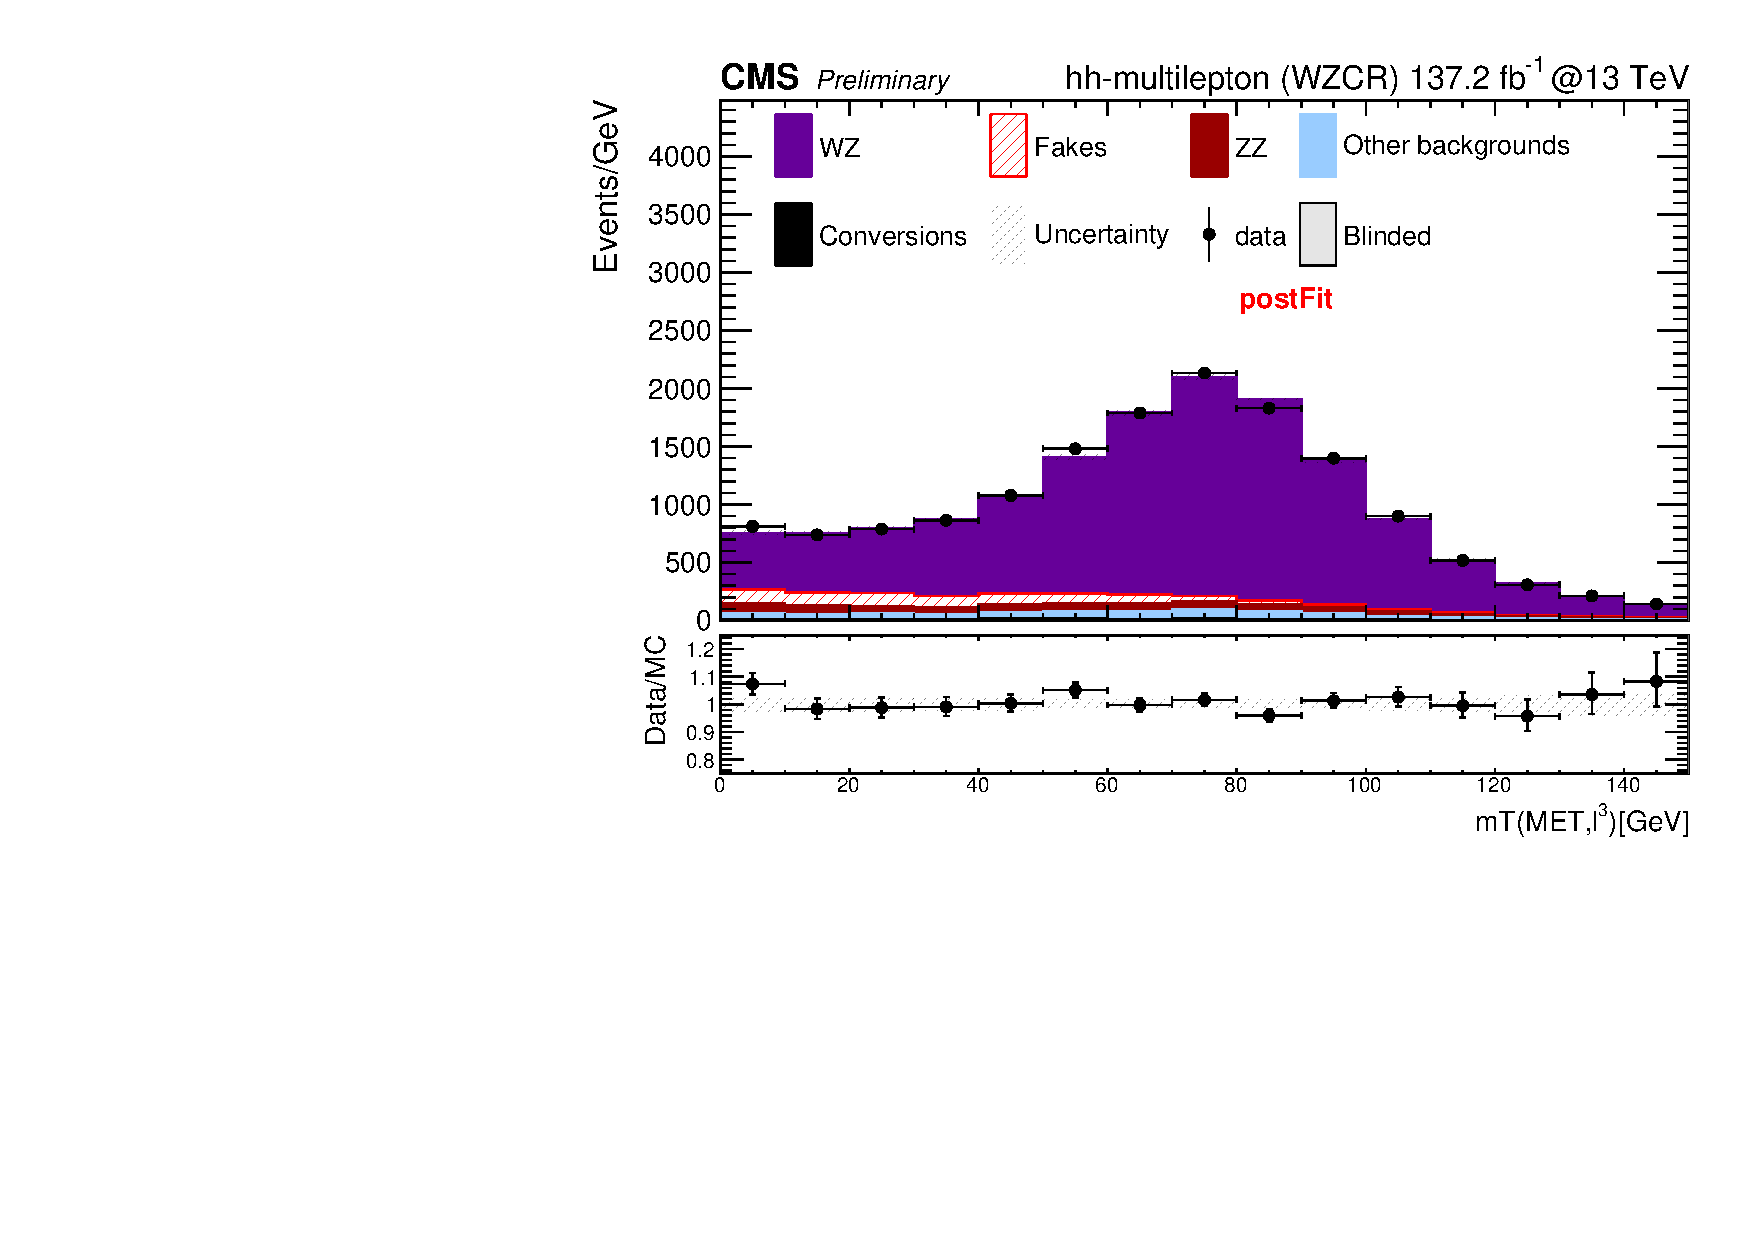
\includegraphics[width=\cmsFigWidth]{figures/postFitPlots/WZ.pdf}
  %% \centering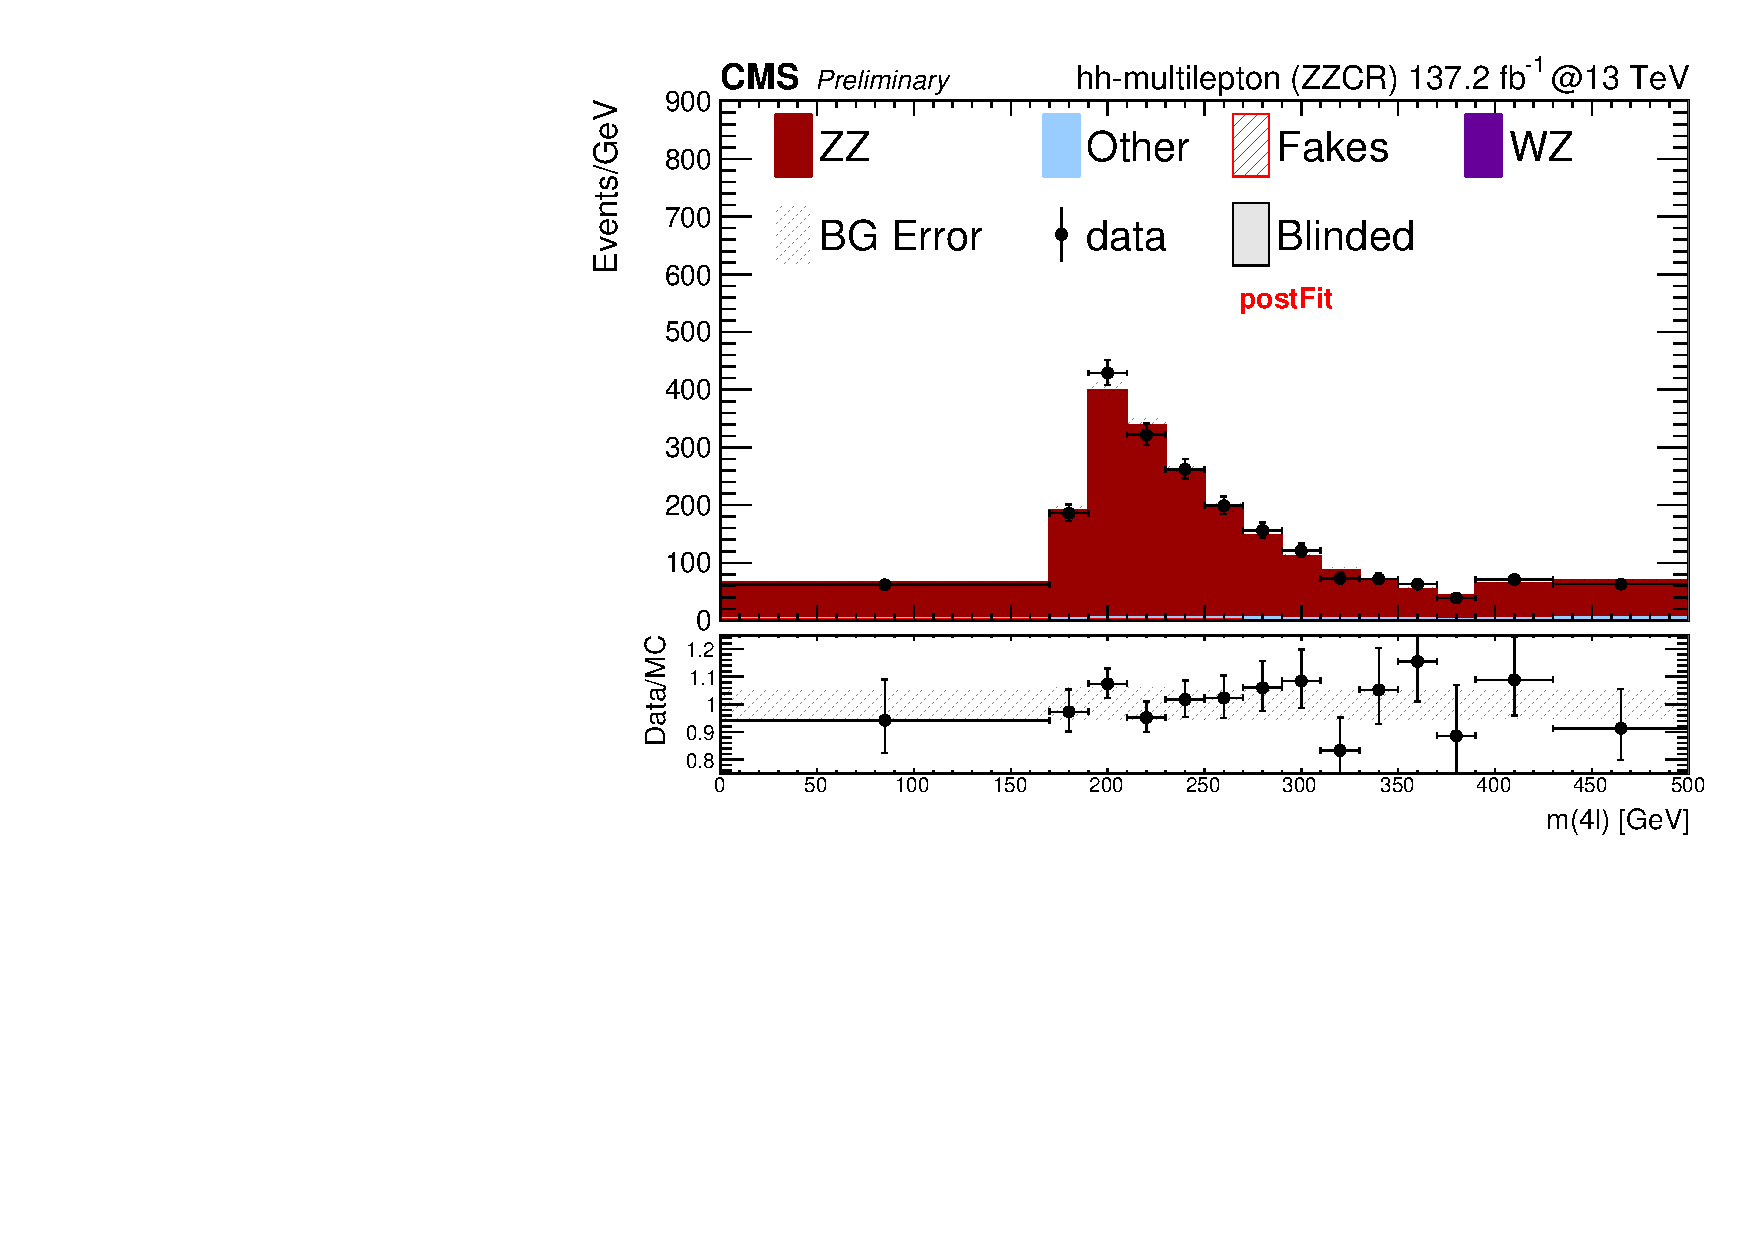
\includegraphics[width=\cmsFigWidth]{figures/postFitPlots/ZZ.pdf}
  \caption{
    Distribution in the observable $\mT$ in the \threeLeptonCR (left) and in the observable $m_{4\Plepton}$ in the \fourLeptonCR (right).
    The distributions expected for the $\PW\PZ$ and $\PZ\PZ$ as well as for other background processes
    are shown for the values of nuisance parameters obtained from the ML fit described in Section~\ref{sec:results}.
  }
  \label{fig:postfitPlotsCR}
\end{figure}

Overlap between irreducible and reducible backgrounds and between the different types of reducible backgrounds,
which would cause the double-counting of background contributions,
is avoided by categorizing each simulated event as either irreducible background or as fakes, flip, or conversion background.
The different types, or classes, of backgrounds are made mutually exclusive by ranking them in priority and assigning each simulated event to the class of highest priority for which it qualifies.
The ranking, in order to decreasing priority, is: fakes, flip, conversion, and irreducible background.
Thus, a simulated event selected in the \threeLeptonOneTau search category, which contains a reconstructed $\tauh$ that is due to the misidentification of a jet,
a reconstructed electron that is due to a photon conversion, and two genuine prompt leptons is categorized as fakes background, for example.
The evaluation of the category is based on matching reconstructed $\Pe$, $\PGm$, and $\tauh$ to their MC truth.
Electrons and muons that are misidentified as $\tauh$ and $\tauh$ that are misidentified as $\Pe$ or $\PGm$ are treated as non-fakes.


\subsection{Estimation of the ``fakes'' background}
\label{sec:backgroundEstimation_fakes}

The background from misidentified leptons and $\tauh$ is estimated using the fake-factor (FF) method~\cite{Sirunyan:2018shy}.
An estimate for the fake background contribution in the SR of each search category is obtained
by selecting a sample of events that satisfy all selection criteria of the SR for the respective search category,
except that the $\Pe$, $\PGm$, and $\tauh$ are required to pass the loose selections instead of the tight ones.
The sample of events thus obtained is referred to as the application region (AR) of the FF method.
Overlap between AR and SR is avoided by excluding from the AR those events in which all leptons and $\tauh$ satisfy the tight selections.

The estimate for the fake background contribution in the SR is obtained by applying suitably chosen weights to the events selected in the AR.
The weights, denoted by the symbol $w$, are given by the expression:
\begin{equation}
w = (-1)^{n+1} \, \prod_{i=1}^{n} \, \frac{f_{i}}{1 - f_{i}}\,
\label{eq:FF_weights}
\end{equation}
where the product extends over all $\Pe$, $\PGm$, and $\tauh$
that pass the loose, but fail the tight selection criteria,
and $n$ refers to the total number of such leptons and $\tauh$.
The symbol $f_{i}$ corresponds to the probability for an $\Pe$, $\PGm$, or $\tauh$ that passes the loose selection to also pass the tight one.
The contributions of irreducible backgrounds to the AR are subtracted based on the MC expectation of such contributions.

The probabilities $f_{i}$ for leptons are measured in multijet events, separately for electrons and muons, as described in Ref.~\cite{Sirunyan:2020icl},
and are parametrized by \pt and $\eta$ of the lepton candidate.

The $f_{i}$ for $\tauh$ are measured using $\Zmm$+jets events.
The events are selected by requiring the presence of two muons of opposite charge and mass $60 < m_{\Pgm\Pgm} < 120\GeV$,
passing the tight muon selection.
The leading and subleading muons are required to pass $\pt$ cuts of $25$ and $15\GeV$.
The events are further required to contain at least one $\tauh$ candidate that passes the loose $\tauh$ selection.
Events containing either one jet that passes the tight $\Pbottom$-tagging WP or two jets that pass the loose WP are vetoed to remove $\ttbar$ background.
The event sample thus selected is referred to as the measurement region (MR) of the FF method.
The measured probabilities $f_{i}$ for $\tauh$ are parametrized by \pt and $\eta$ of the $\tauh$ candidate.


\subsection{Estimation of the ``flips'' background}
\label{sec:backgroundEstimation_flips}

The flips background in the $\twoLeptonssZeroTau$ channel is estimated using the method described in Ref.~\cite{Sirunyan:2020icl}.
The procedure for estimating the flips background is similar to that for estimating the fakes background.
A sample of events passing all selection criteria of the SR of the $\twoLeptonssZeroTau$ channel, 
except that both leptons are required to be of OS instead of SS charge, 
are selected and assigned appropriately chosen weights.
The latter are given by the sum of the probabilities for the charge of either lepton to be mismeasured.
The probability for the charge of electrons to be mismeasured, referred to as the electron charge misidentification rate,
is determined using $\Zee$ events.
The probability for mismeasuring the charge of muons is negligible~\cite{Sirunyan:2020icl}.

\section{Systematic uncertainties}
\label{sec:systematicUncertainties}

When measuring the $\HH$ cross section for various signal models,
there are multiple sources of systematic uncertainty which affect
the predicted yields and BDT discriminator output shapes for different
sources of signal and background.
These uncertainties are either theoretical, affecting the predicted cross
section or decay kinematics of the collision process, or experimental,
accounting for possible mis-modeling of reconstructed objects.
Systematic uncertainties may either be treated as correlated or
uncorrelated among the three years of data taking, and among the
different signal and background processes.

The SM prediction for the inclusive $\HH$ production cross section
via gluon fusion at $13\TeV$ center-of-mass collision energy is
$31.05^{+1.14}_{-1.196}\fb$ at NNLO accuracy, with missing higher
orders and undertainties in the proton parton density function (PDF)
and strong coupling $\alpha_{s}$ driving the uncertainty. %%~\cite{FIXME}
The Vector Boson Fusion $\HH$ process has a cross section of
$1.276\pm0.027\fb$, with PDF and $\alpha_{s}$ accounting for most of
the uncertainty. %%~\cite{FIXME}
The predicted Higgs boson decay branching fractions to $\PW\PW$,
$\PGt\PGt$, and $\PZ\PZ$ have relative uncertainties of $1.54\%$,
$1.65\%$, and $1.54\%$, respectively. %%~\cite{FIXME}
%% https://github.com/HEP-KBFI/CombineHarvester/blob/master/ttH_htt/configs/list_syst_HH.py#L142-L161
Alternate $\HH$ predictions are generated with the renormalization
and factorization scales varied up and down by a factor of two, which
constitute an uncertainty on the BDT output shape and event yields
in each signal category, due to decay product acceptance in the detector.
All theoretical uncertainties on signal $\HH$ production are correlated
across all three years and among the selected event categories.
Their primary impact is on the measurement of the $\HH$ production
cross section as a ratio of the SM prediction.
Only the acceptance uncertainty affects the $\HH$ inclusive cross
section measurement, and none of these uncertainties impact the
limits on resonant $\HH$ production or $\HH$ production in EFT scenarios.
%% NOTES: Branching uncertainties in AN definitely incorrect, need to
%%        confirm correlation scheme, not clear if norm/fact is a "shape-only"
%%        uncertainty given that it is included in inclusive xsec uncertainty.
%%        Double-check SM mu vs. SM xsec vs. BSM usage of uncertainties.

Background processes which produce enough ``prompt'' electrons, muons,
and $\PGt$ leptons to match the selection criteria in one or more
event categories have theoretial uncertainties associated with their
production cross sections.
The relative uncertainties in the dominant $\PW\PZ$ and $\PZ\PZ$ background
cross sections are $2.1\%$ and $6.3\%$, respectively. %% ~\cite{FIXME}
Sub-dominant single Higgs production cross section uncertainties range
from $2$-$9\%$ for gluon fusion, VBF, and associated production with a
$\PW$ or $\PZ$ boson. %% ~\cite{FIXME}
Reducible backgrounds with one or two top quarks produced in association
with a $\PW$, $\PZ$, or $\PH$ boson have cross section uncertainties that
range from $8$ to $15\%$. %% ~\cite{FIXME}
The normalization for extremely rare backgrounds not mentioned above
(e.g.~triple boson or four top quark production) is given a $50\%$ uncertainty.
Background events where at least one reconstructed lepton or $\tauh$
originates from a photon conversion are assigned a $30\%$ yield uncertainty.
Theoretical uncertainties affecting background cross sections are treated
as uncorrelated among different physics processes, but correlated across
the different years and among all seven signal categories.
%% NOTES: Confirm correlation scheme outlined above.  Are "photon conversion"
%%        events all lumped together regardless of underlying physics process?

The prediction for events with at least one selected non-prompt,``fake'',
or charge mis-assigned lepton or $\tauh$ entering the signal region
(described in Sec.~\ref{sec:backgroundEstimation} is assigned a $30\%$
normalization uncertainty in most categories.
Since the $\lllt$ and $\lttt$ categories use modified $\tauh$ selection criteria
(Sec.~\ref{sec:eventReconstruction}), this uncertainty is raised to $50\%$.
An additional uncertainty on the BDT output shape in each category is
evaluated for events with a non-prompt or ``fake'' lepton or $\tauh$
by means of a ``closure test'' in MC simulation.
Events passing all signal selection criteria are compared to those
with at least one lepton or $\tauh$ failing the ``tight'' identification,
scaled according to the ``fakeable-to-tight'' method described in
Sec.~\ref{sec:backgroundEstimation}.
The ratio of these two shapes is fit with a linear function, which
is convoluted with the non-prompt and ``fake'' background prediction
from the data to serve as an uncertainty on the BDT output shape
for these events in the signal region.
The systematic uncertainties associated with the non-prompt and ``fake''
lepton prediction are treated as uncorrelated amongst the different
years, while the uncertainty on charge mis-assignment probability
is correlated.
%% NOTES: Are non-prompt yields correlated at all between categories?
%%        State level of closure in fake/flip yields and shape from MC closure, control regions?

Uncertainties in the modeling of the trigger and object reconstruction
affect all signal and background processes estimated using MC simulation.
Trigger efficiencies are for events with at least two leptons are compared
between data and MC in multi-lepton control regions enriched in the $\ttbar$,
$\PW\PZ$, and $\PZ\PZ$ background processes, as a function of lepton flavor,
$\pt$, and $\eta$.
This results in a small $\pt$ dependent uncertainty correlated between the
$\llss$ and $\lltt$ categories, and a $1\%$ normalization uncertainty
correlated among the $\lllnot$, $\lllt$, and $\llll$ categories.
For the $\tttt$ and $\lttt$ categories, the data-to-simulation agreement in
trigger efficiency is computed using an independent set of events in data,
and parameterized as a function of the $\tauh$ $\pt$, $\eta$, $\phi$, and
reconstructed decay mode. %%~\cite{FIXME}
The trigger uncertainties for these two categories are treated as uncorrelated.
All systematic uncertainties related to trigger modeling are correlated
across different physics processes, but uncorrelated amongst the three years.
%% NOTES: Check which control regions are used for leptons, and pt/eta/other dependence.
%%        Verify that trigger efficiency scale factors are not applied to non-prompt.

The uncertainties in reconstruction and identification efficiency for electrons,
muons, and $\tauh$ have been measured in $\PZ$ boson enriched regions in data
for each level of identification criteria (``loose'', ``fakeable'', and ``tight''),
and are applied to each event as a function of lepton $\pt$ and $\eta$, or
$\tauh$ $\pt$ and reconstructed decay mode.
The reconstructed $\tauh$ energy 

\section{Results}
\label{sec:results}

The data selected in the seven search categories and in the two
control regions enriched in $\PW\PZ$ and $\PZ\PZ$ backgrounds
is tested against multiple $\HH$ production hypotheses,
as described in Section~\ref{sec:introduction}: the SM prediction;
variations of the SM coupling strength modifiers
$\kappal$, $\kappat$, $\kappaV$, and $\kappaVV$;
the effective couplings $\cg$, $\cgg$, and $\ctwo$ in the EFT approach;
and resonant production from the decay of heavy particles of either spin-0 or
spin-2 particles and masses $m_{\X}$ in the range $250 \leq m_{\X} \leq 1000\GeV$.
In each case, the entire dataset is fit simultaneously to a model
composed of the background prediction (with uncertainties),
and the $\HH$ signal hypothesis under consideration.

The SM ``signal strength'' parameter is defined as
$\mu = \sigma(\HH)_{\textrm{best fit}} / \sigma(\HH)_{\textrm{SM}}$,
and modifies the expected signal yield by the same proportion in each category.
By contrast, variations in the $\kappa$ modifiers may affect the signal yields in each
category differently, and also change the BDT discriminant output shape for $\HH$ events.
The twelve benchmark scenarios spanning combinations of $\kappal$, $\kappat$,
$\cg$, $\cgg$, and $\ctwo$ values in the EFT parameter space each correspond to
different signal kinematics, so the $\HH$ production cross section $\sigma$
for each point is measured separately.
Similarly, signal efficiency and BDT discriminant output shape vary dramatically for different
resonant masses, and thus a separate measurement is performed for each mass and spin hypothesis.
The SM signal strength and $\kappa$ measurements are performed using the output of the BDT classifier
that has been trained for non-resonant $\HH$ production and setting the $13$ binary inputs to the values corresponding to the SM case.
When setting limits on the $12$ different EFT benchmark scenarios, the binary inputs are set to the value corresponding to the respective scenario.
In case of resonant $\HH$ production, the real-value BDT input that corresponds to the mass of the heavy particle $\X$ 
is set to the $m_{\X}$ value for which the limit is computed.

The SM signal strength is measured using a profile likelihood test
statistic~\cite{Cowan:2010js}, with systematic uncertainties treated as nuisance
parameters $\theta$ in a modified frequentist approach~\cite{ATL-PHYS-PUB-2011-011}.
Statistical uncertainties on the distributions in the BDT discriminant output for the $\HH$ signal and for background processes
are taken into account using the approach detailed in Ref.~\cite{Barlow:1993dm}.
The likelihood ratio $q_{\mu}$ for a fixed ``test'' signal strength value $\mu$ is:
\begin{linenomath}
\begin{equation*}
  \begin{aligned}
    q_{\mu}  &  = -2 \Delta \ln \mathcal{L} = \ln \frac{\mathcal{L}(\mathrm{data}|\mu,\hat{\theta}_{\mu})}{\mathcal{L}(\mathrm{data}|\hat{\mu},\hat{\theta})}
  \end{aligned}
\end{equation*}
\end{linenomath}
where $\hat{\mu}$ and $\hat{\theta}$ are the signal strength and nuisance
parameter values which give the maximum value of the likelihood function $\mathcal{L}$
for the given set of data, and $\hat{\theta}_{\mu}$ is the set of nuisance
parameter values which maximize $\mathcal{L}$ for the fixed $\mu$ value.
The 95\% confidence interval includes all values of $\mu$ for which $q_{\mu} < 1.96$,
within approximately two standard deviations of the global best-fit value ($q_{\hat{\mu}} = 0$).
The SM coupling strength modifiers and the cross sections for the various $\HH$ production hypotheses
are measured by profiling values of $\kappa$ and $\sigma$, respectively,
relative to $\hat{\kappa}$ and $\hat{\sigma}$.
Theoretical and experimental uncertainties affecting the signal and
background yields or the shape of the BDT discriminant output distributions are fully
correlated across all years, event categories, and discriminant bins,
except as noted in Section~\ref{sec:systematicUncertainties}.

The fits to all BDT output discriminant distributions in data are consistent with the
SM background prediction in all selection categories, within statistical and systematic uncertainties.
The observed 95\% confidence level (CL) upper limit on the SM $\HH$ production cross section
amounts to $X.XX$~\pb ($Y.YY$ times the SM prediction), compared to an
expected limit of $Z.ZZ$~\pb.
The latter quantifies the sensitivity of the analysis in the absence of a signal.
These limits are shown in Fig.~\ref{fig:HH_limits_SM} [TODO: Create],
for individual categories and for the combined result.
The \lttt and \lllnot categories provide the strongest individual
constraints on the SM $\HH$ cross section.

\begin{figure}
  \centering
  %% \includegraphics[width=0.45\textwidth]{figures/SM_limits.pdf}
  \caption{
    Observed and expected 95\% CL limits on the SM $\HH$ production cross section
    for the CMS Run~2 dataset of 137.2\fbinv, for both individual event categories
    and for their combination.
  }
  \label{fig:HH_limits_SM}
\end{figure}

The 95\% CL interval for the $\PHiggs$ boson trilinear self-coupling strength modifier
is measured to be $X.XX < \kappal < Y.YY$, where the upper limit is the [second]
strongest constraint on this fundamental SM parameter to date~\cite{Sirunyan:2745738,Sirunyan:2018ayu,2020135103}.
%% CMS Run 2 bbgg limits -3.3 to 8.5, combined 2016 limits -11.8 to 18.8
%% ATLAS combined 2016 limits -5.0 to 12.0
The observed and expected upper limits on the $\HH$ production cross section as a function of
$\kappal$, obtained from the simultaneous fit of all seven search categories, are shown in Fig.~\ref{fig:HH_limits_kLambda}, 
along with limits obtained for each search category individually.
%% Some comment on strongest limits near max/min kLambda values

\begin{figure}
  \centering
  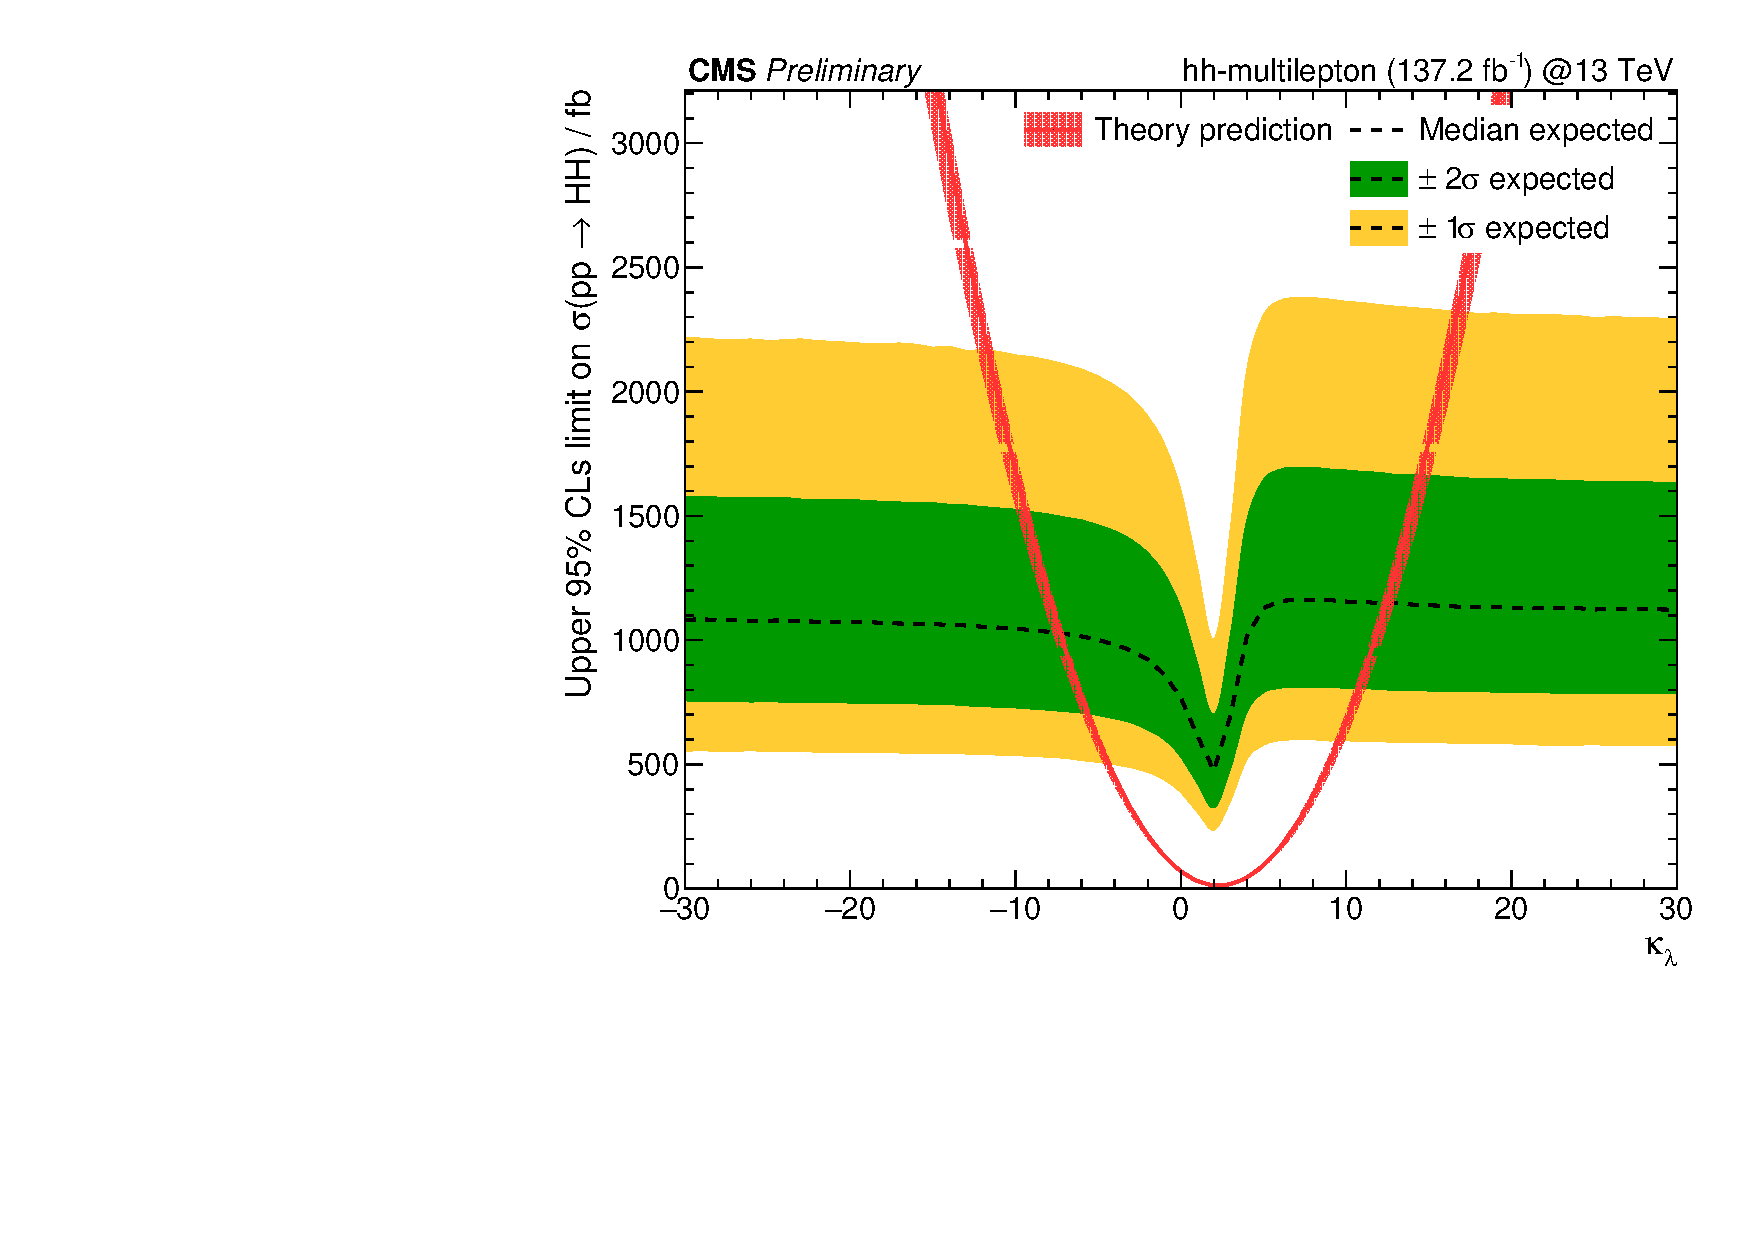
\includegraphics[width=0.45\textwidth]{figures/klscan.pdf}
  \hspace{0.05\textwidth}
  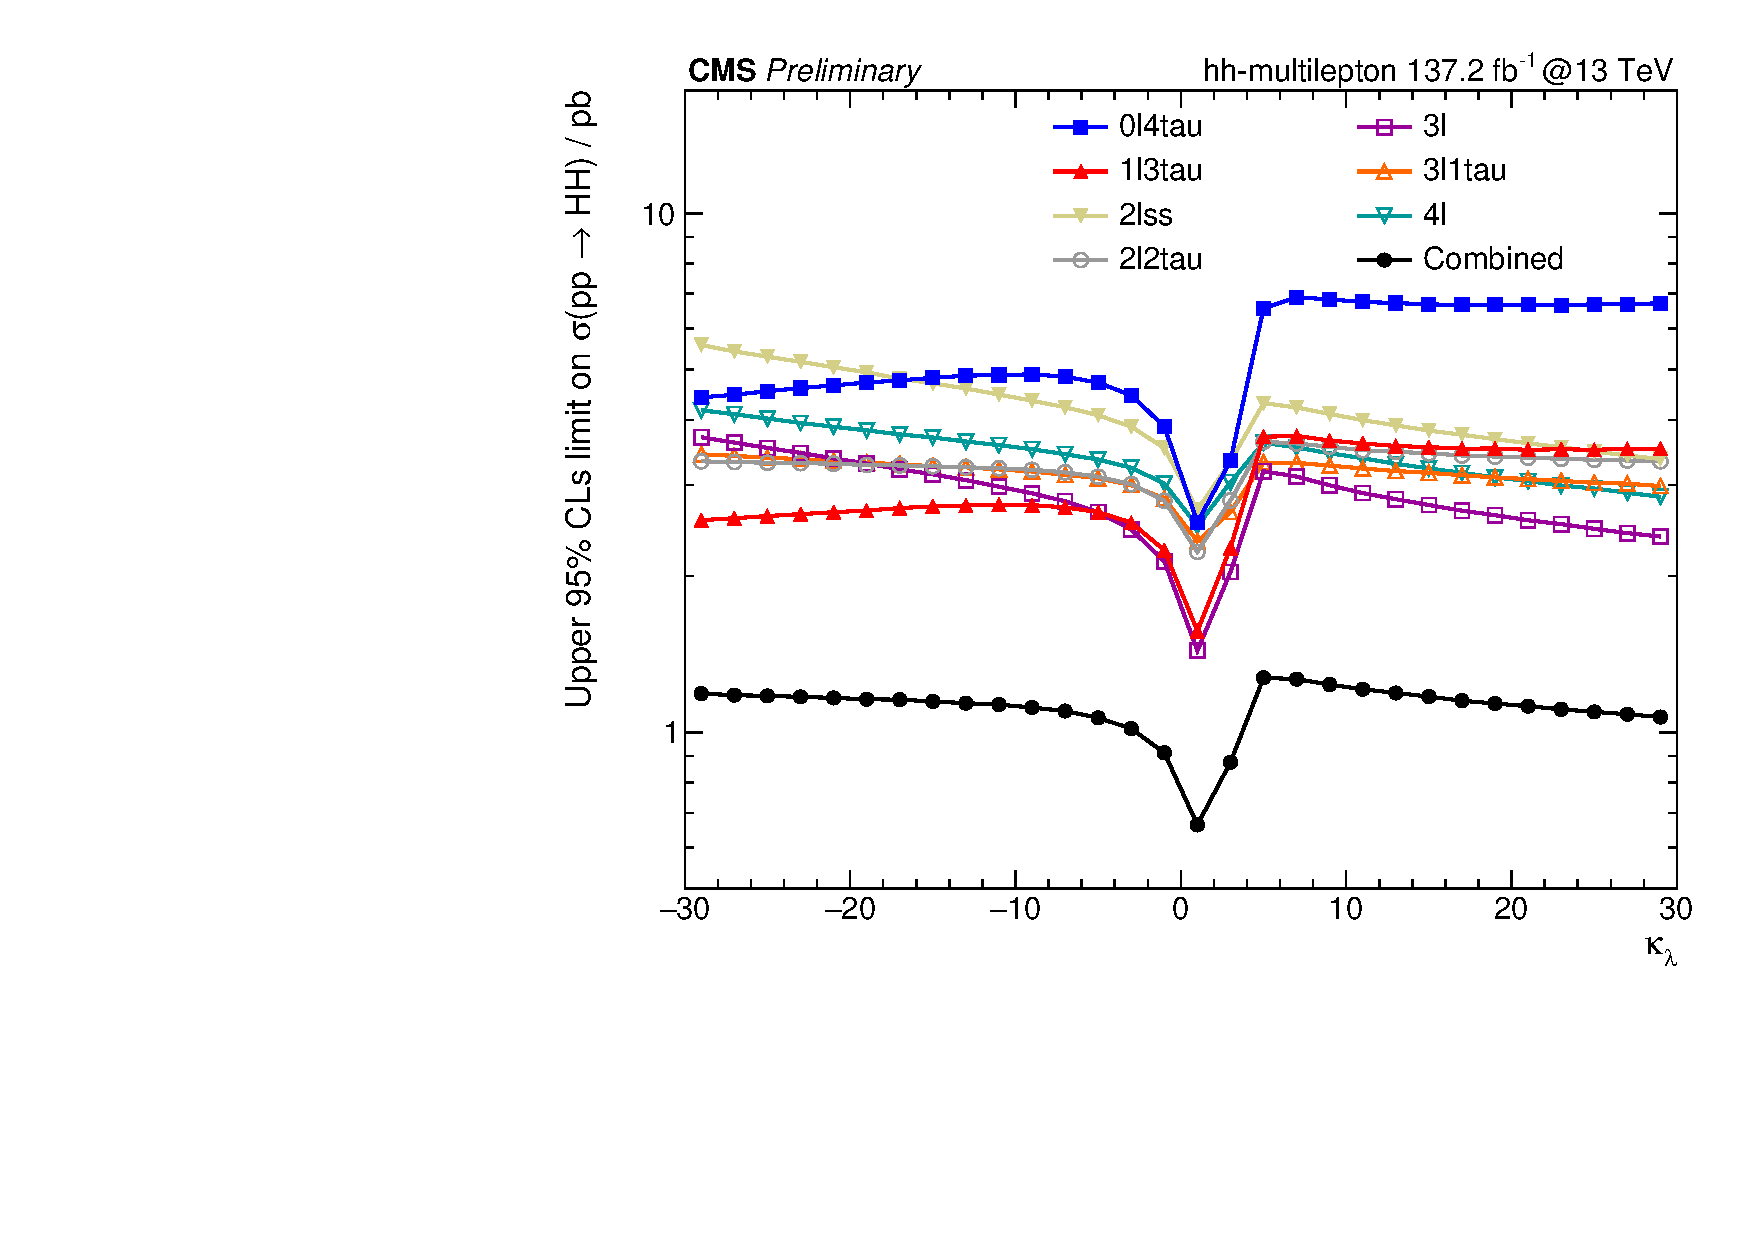
\includegraphics[width=0.45\textwidth]{figures/klMultiscan.pdf}
  \caption{
    Observed and expected 95\% CL limits on the $\HH$ production cross section as
    a function of the Higgs boson self-coupling strength modifier $\kappal$.
    The plot on the left shows the result obtained by combining all seven search categories,
    while the plot on the right shows the limits obtained for each search category separately.  Overlaid is a curve representing the
    predicted $\HH$ production cross section if all SM constants other than
    $\lambda$ have the values predicted in the SM.
  }
  \label{fig:HH_limits_kLambda}
\end{figure}

The observed and expected limits on the $\HH$ production cross section in the
twelve EFT benchmark scenarios are shown in Fig.~\ref{fig:HH_limits_EFT}
and summarized in Table~TODO.
For benchmarks X, Y, and Z, the upper limit cross sections are lower
than for any previous measurement~\cite{Sirunyan:2745738}.
These benchmarks represent models in which the $\HH$ invariant mass is
lower than the SM prediction.  This analysis has a higher signal efficiency
in the low-mass phase space compared to $\HH$ analyses performed in final states with bottom quarks,
because the reconstruction and identification efficiency for low-$\pt$ electrons and muons is higher than for jets of low $\pt$ in CMS.

\begin{figure}
  \centering
  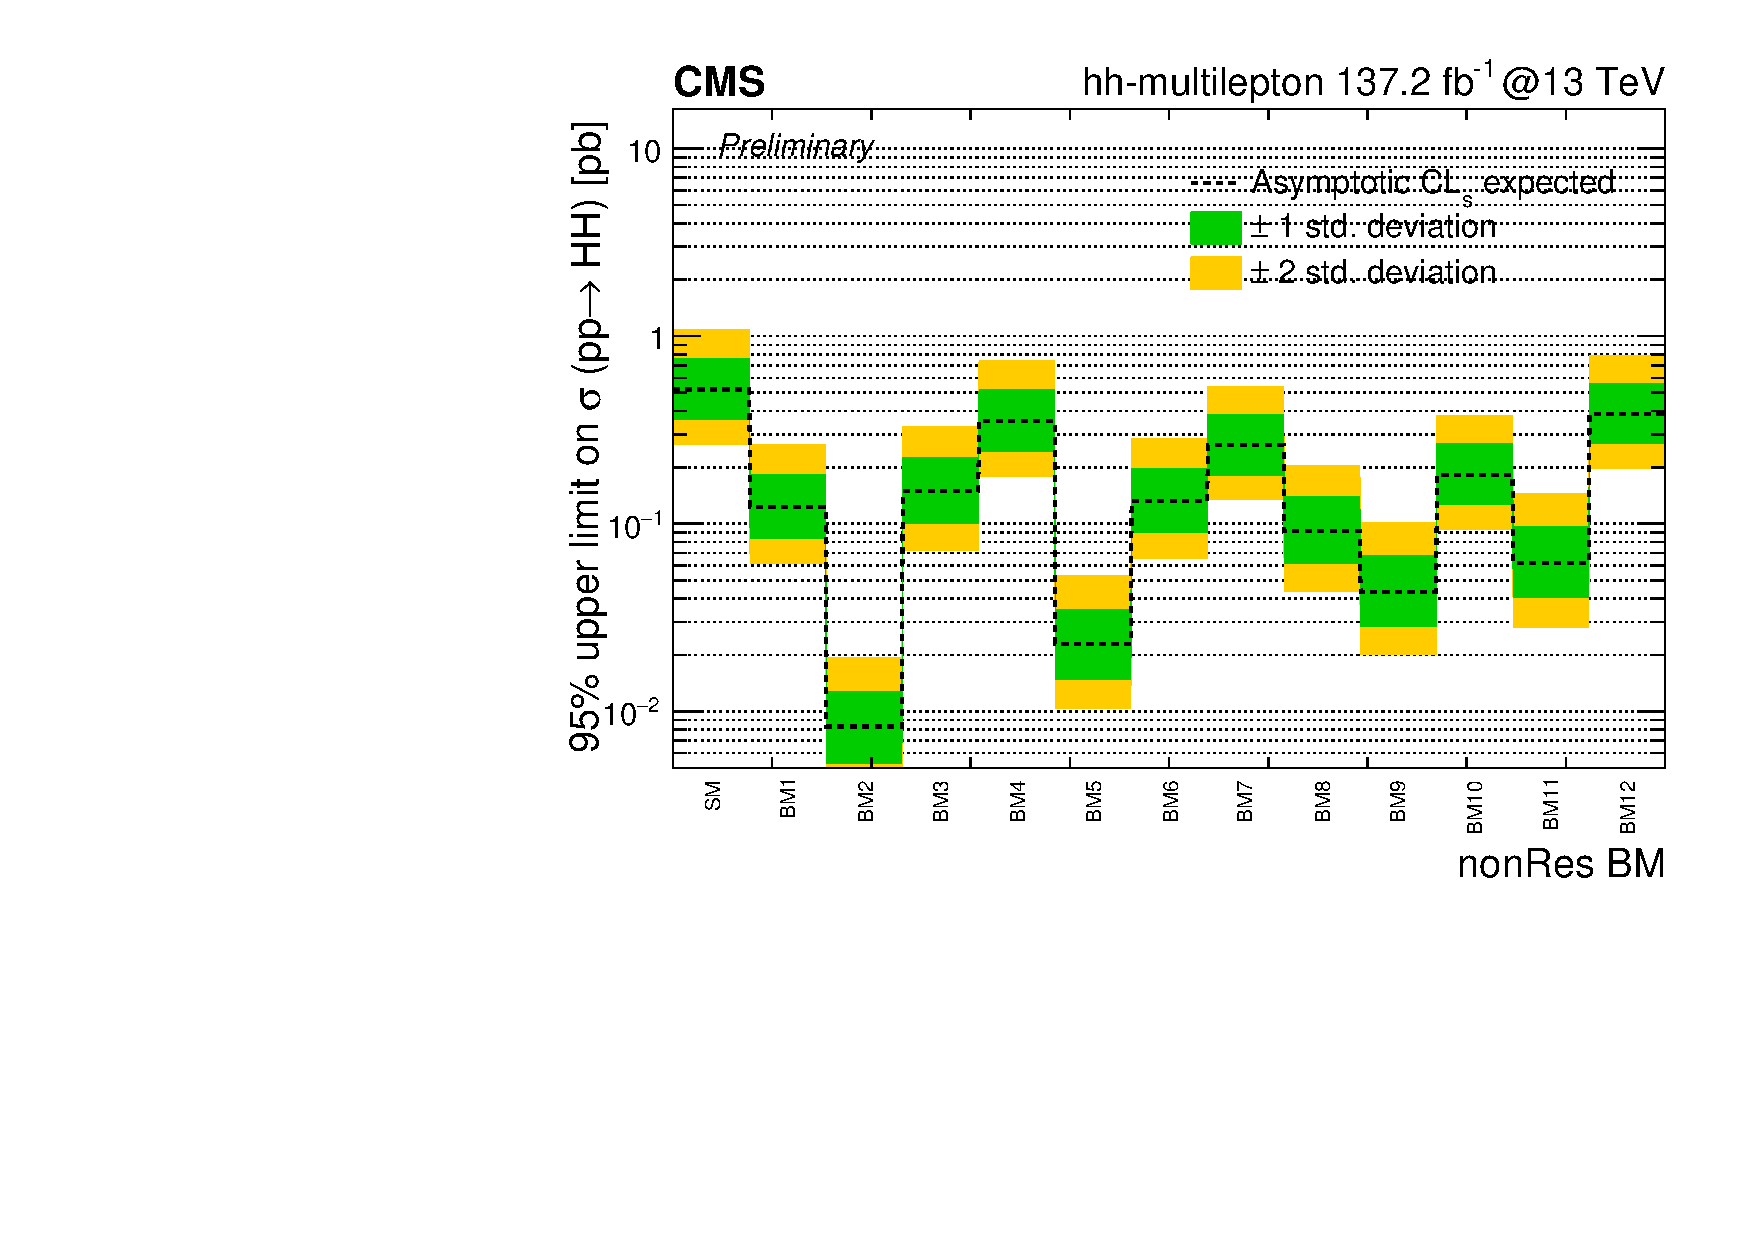
\includegraphics[width=0.45\textwidth]{figures/bmScan_multilepton_RUN2.pdf}
  \hspace{0.05\textwidth}
  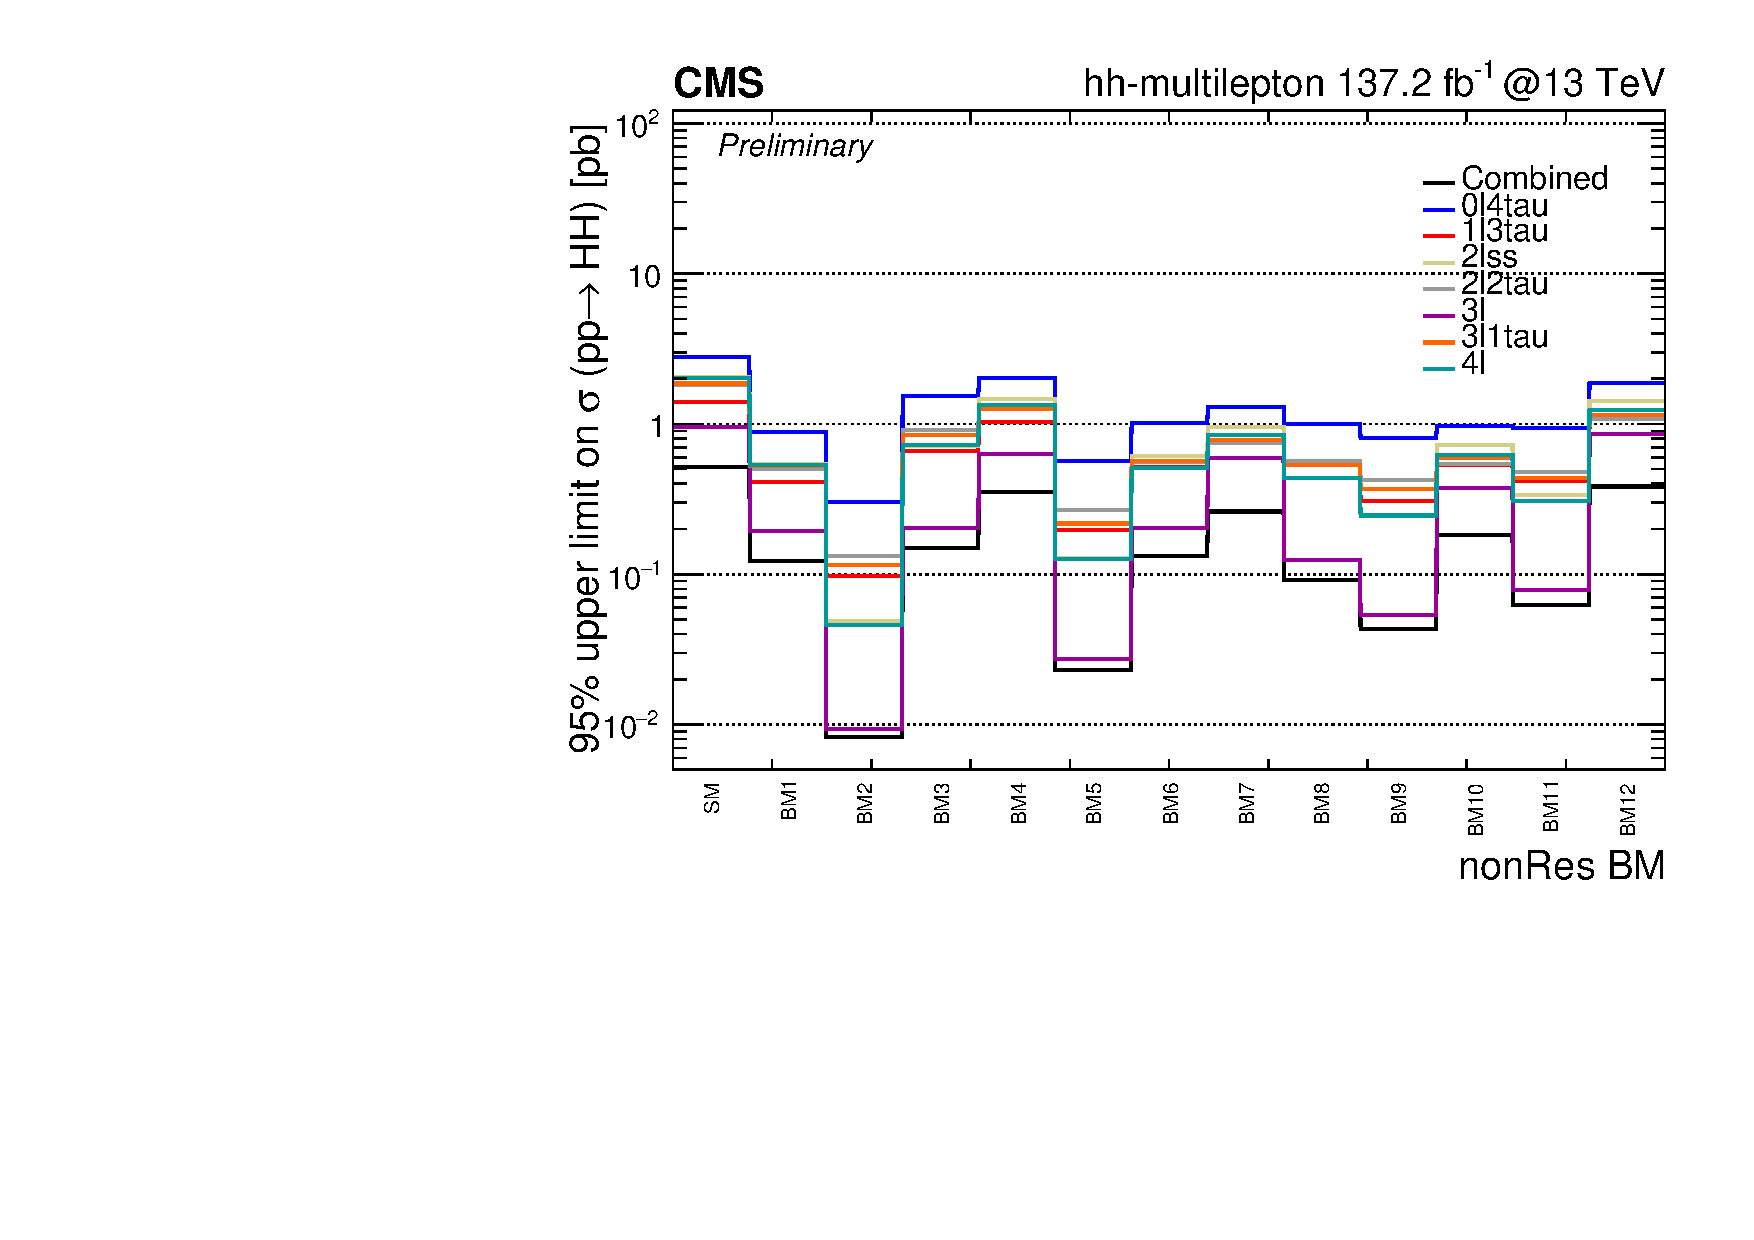
\includegraphics[width=0.45\textwidth]{figures/multiBMScan_multilepton_Run2.pdf}
  \caption{
    Observed and expected 95\% CL limits on the $\HH$ production cross section for
    twelve EFT benchmark scenarios and for the SM.
    The plot on the left shows the result obtained by combining all seven search categories,
    while the plot on the right shows the limits obtained for each search category separately. 
  }
  \label{fig:HH_limits_EFT}
\end{figure}

Figures~\ref{fig:HH_limits_spin0} and \ref{fig:HH_limits_spin2} show the observed and
expected limits on the resonant $\HH$ production cross section as a function of the mass $m_{\X}$ of the particle $\X$,
for spin-0 and spin-2 particles decaying to a $\PHiggs$ boson pair.
Compared to previously published searches for resonant $\HH$
production~\cite{Sirunyan:2018ayu,2020135103},
this analysis has similar sensitivity at very low masses ($250$-$400\GeV$),
owing again to the efficient reconstruction and identification of low-$\pt$ leptons in CMS.

\begin{figure}
  \centering
  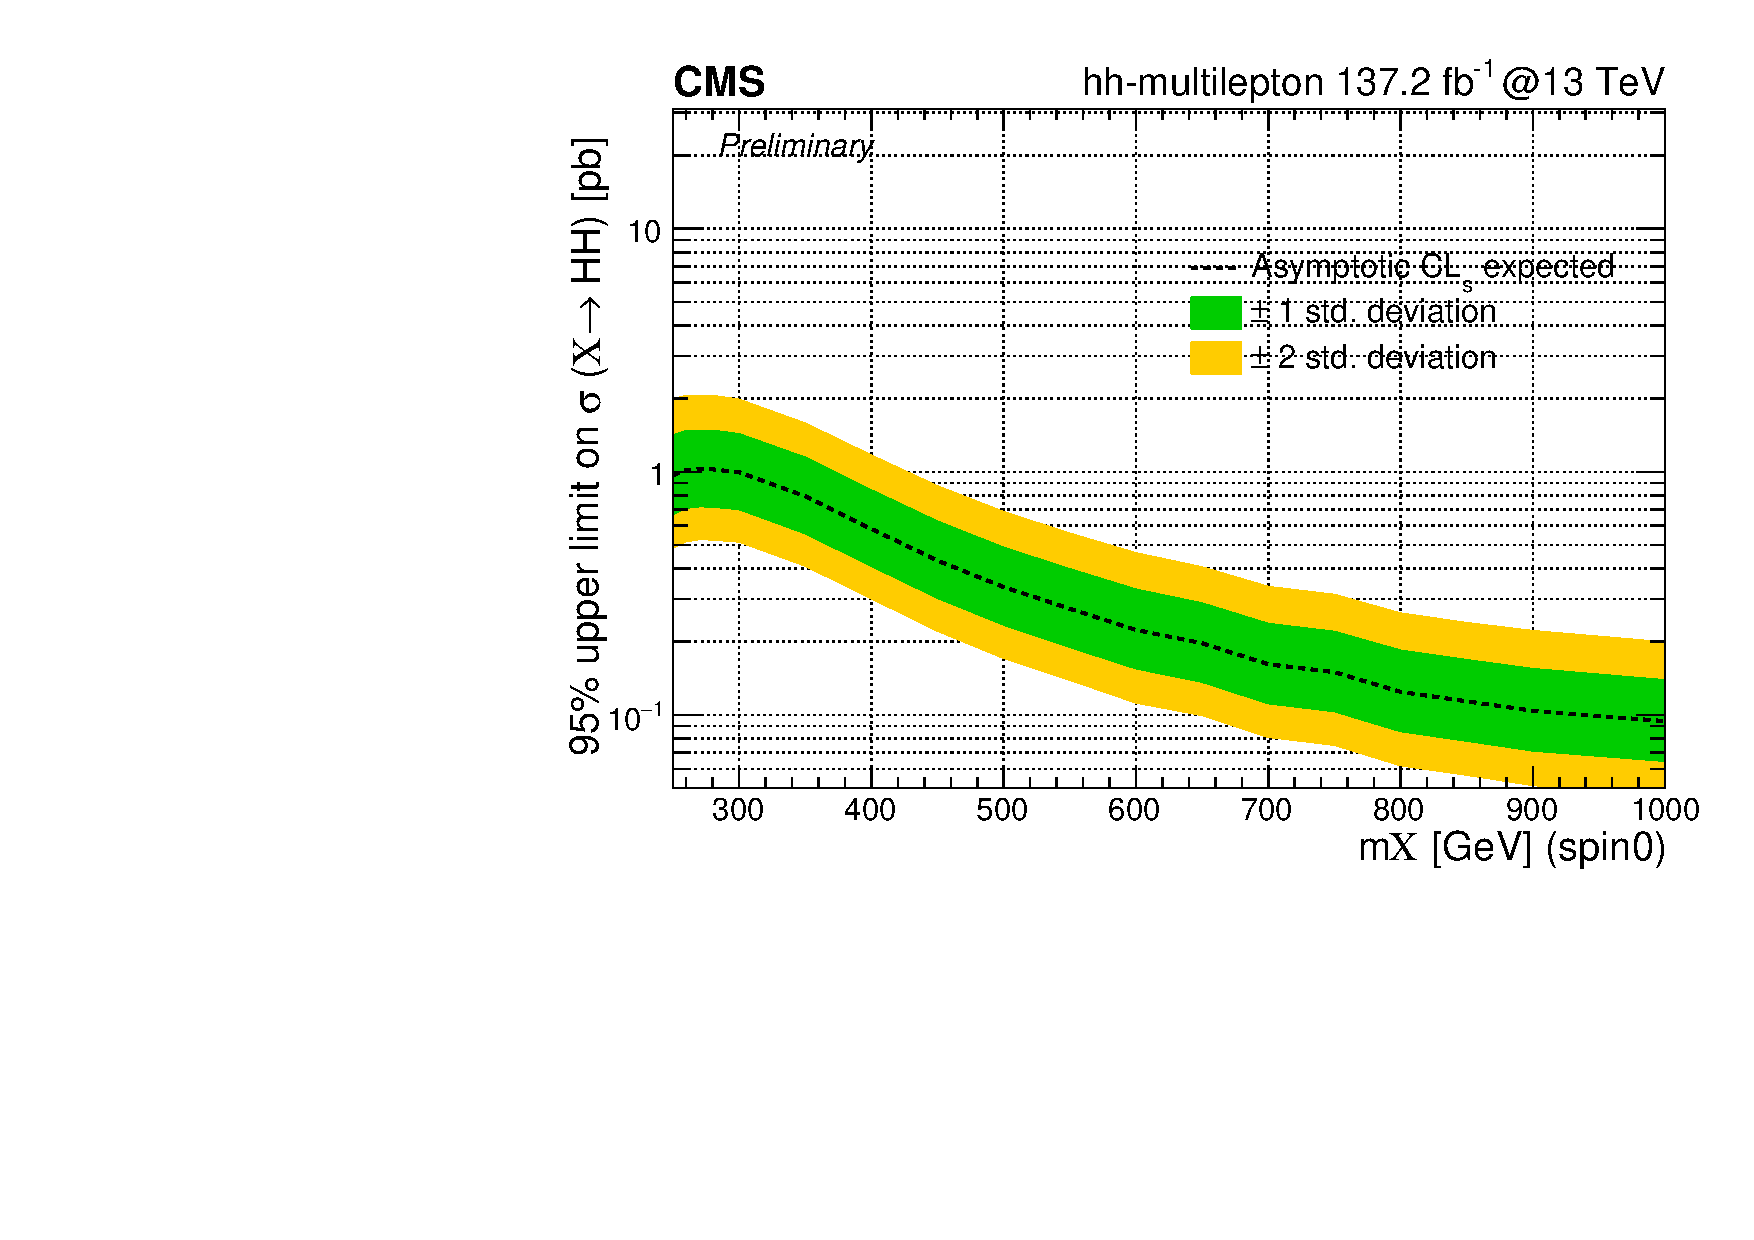
\includegraphics[width=0.45\textwidth]{figures/massScan_spin0_multilepton_RUN2.pdf}
  \hspace{0.05\textwidth}
  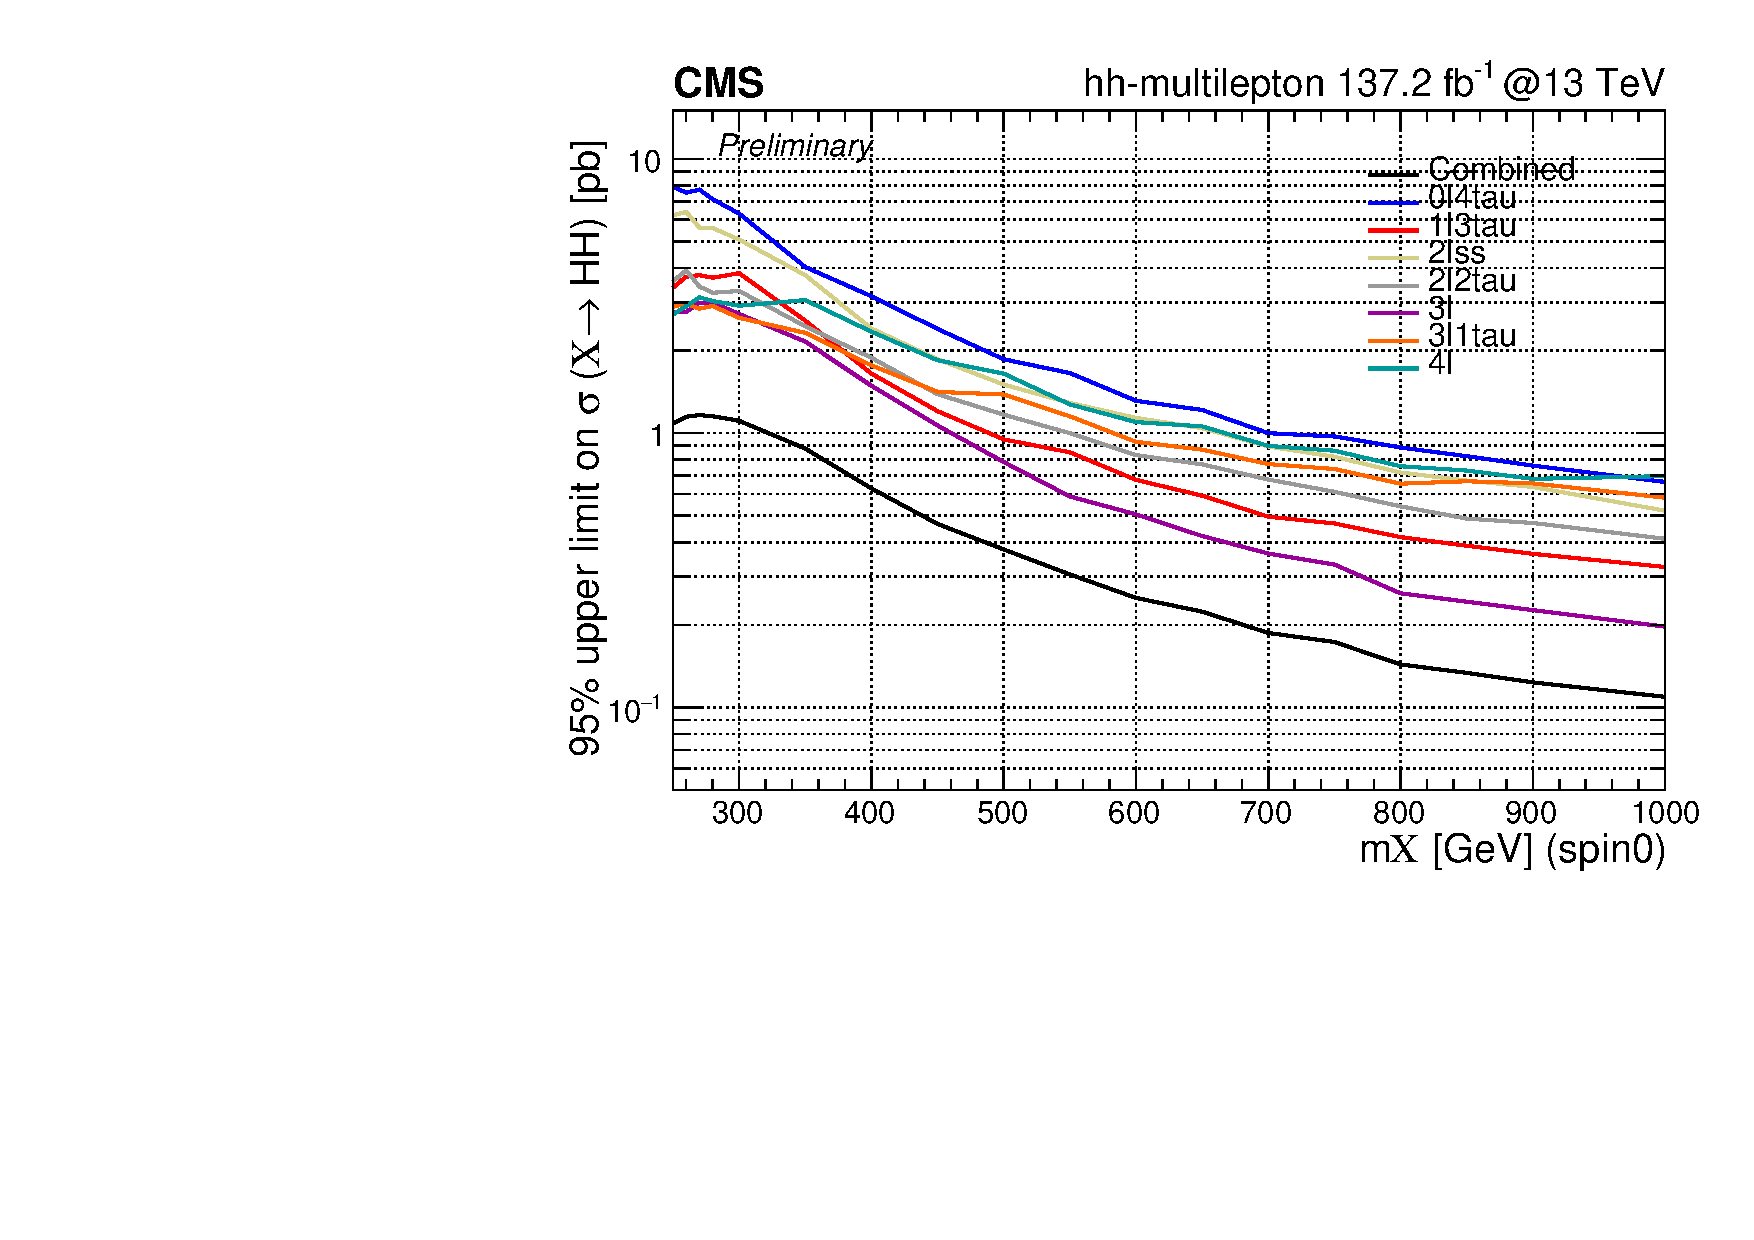
\includegraphics[width=0.45\textwidth]{figures/massMultiScan_spin0_multilepton_Run2.pdf}
  \caption{
    Observed and expected 95\% CL limits on the production of new particles $\X$ of spin $0$ 
    and mass $m_{\X}$ in the range $250 \leq m_{\X} \leq 1000\GeV$, which decay to $\PHiggs$ boson pairs,
    for the combination of all seven search categories (left)
    and for each search category separately (right).
  }
  \label{fig:HH_limits_spin0}
\end{figure}

\begin{figure}
  \centering
  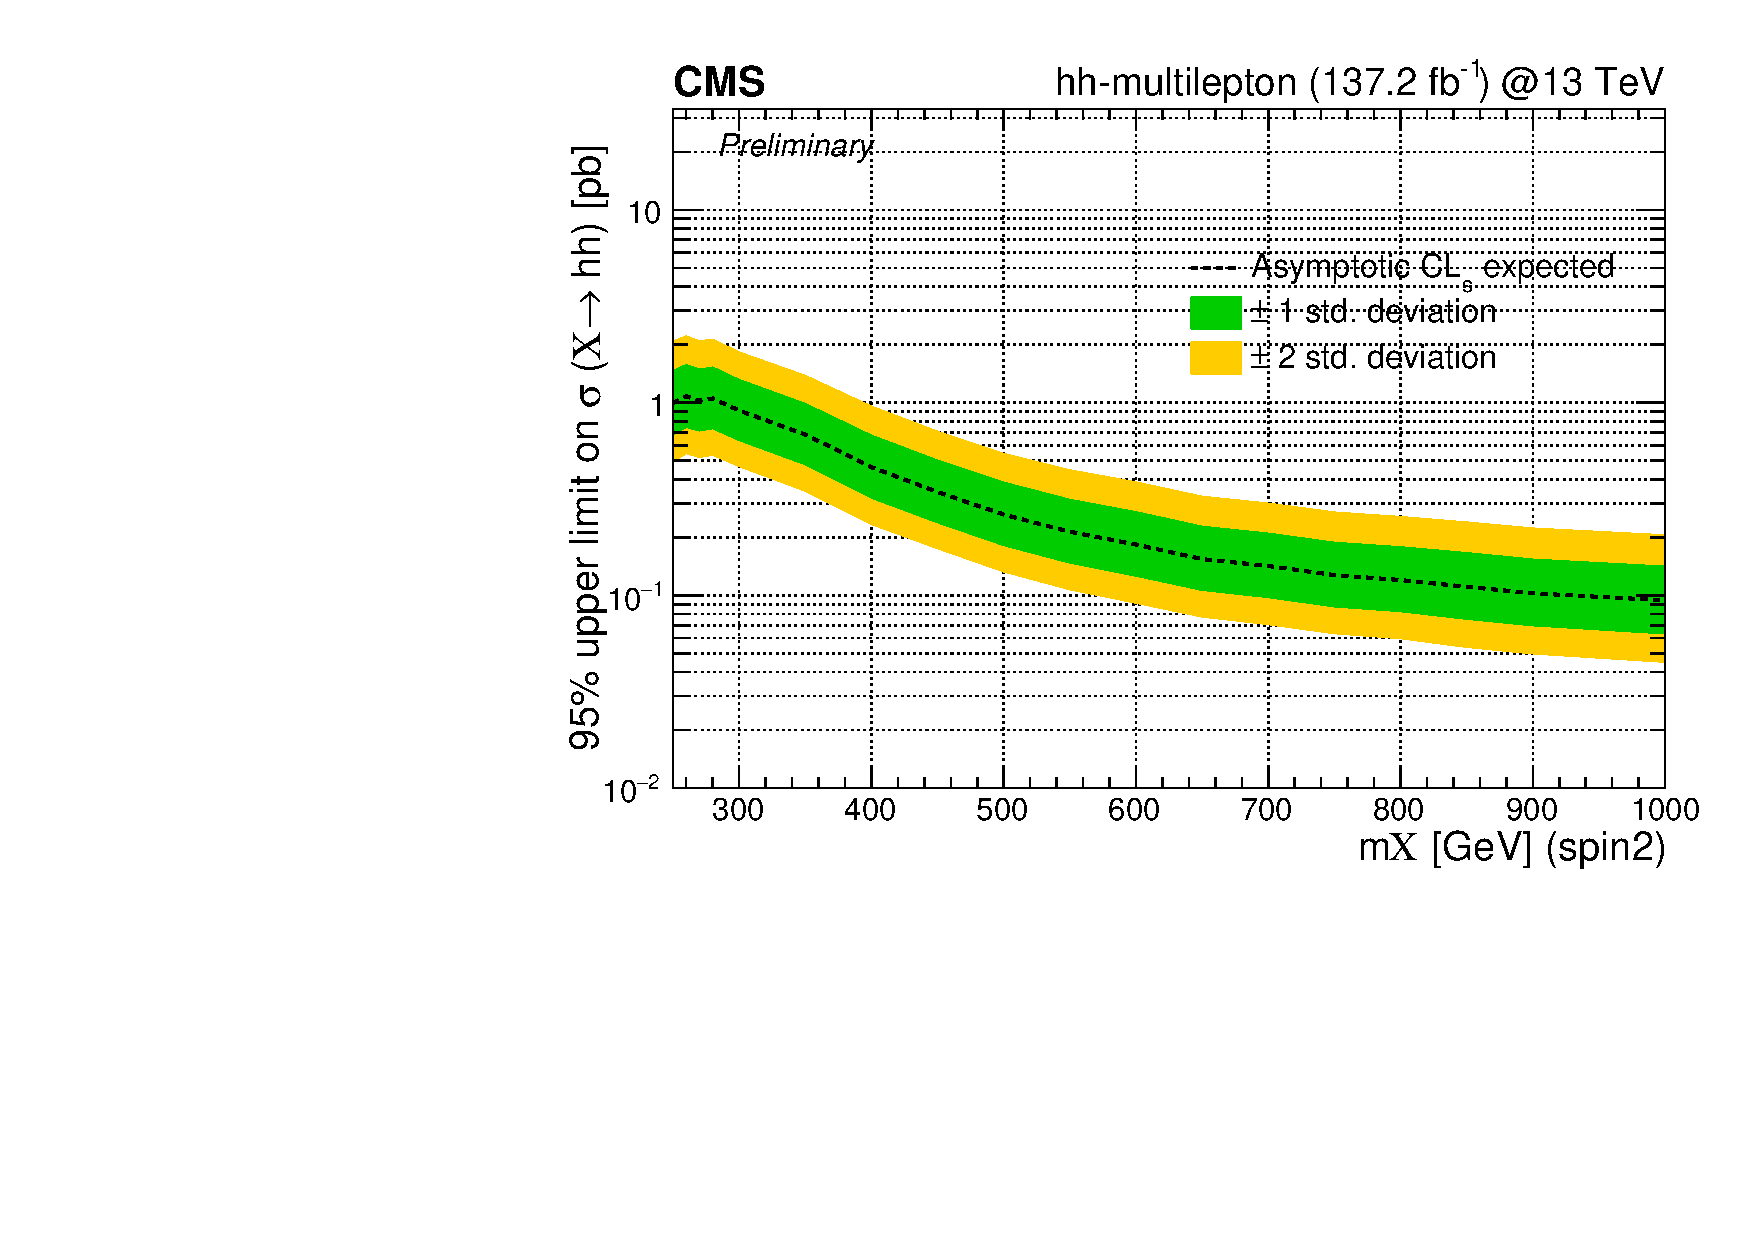
\includegraphics[width=0.45\textwidth]{figures/massScan_spin2_multilepton_RUN2.pdf}
  \hspace{0.05\textwidth}
  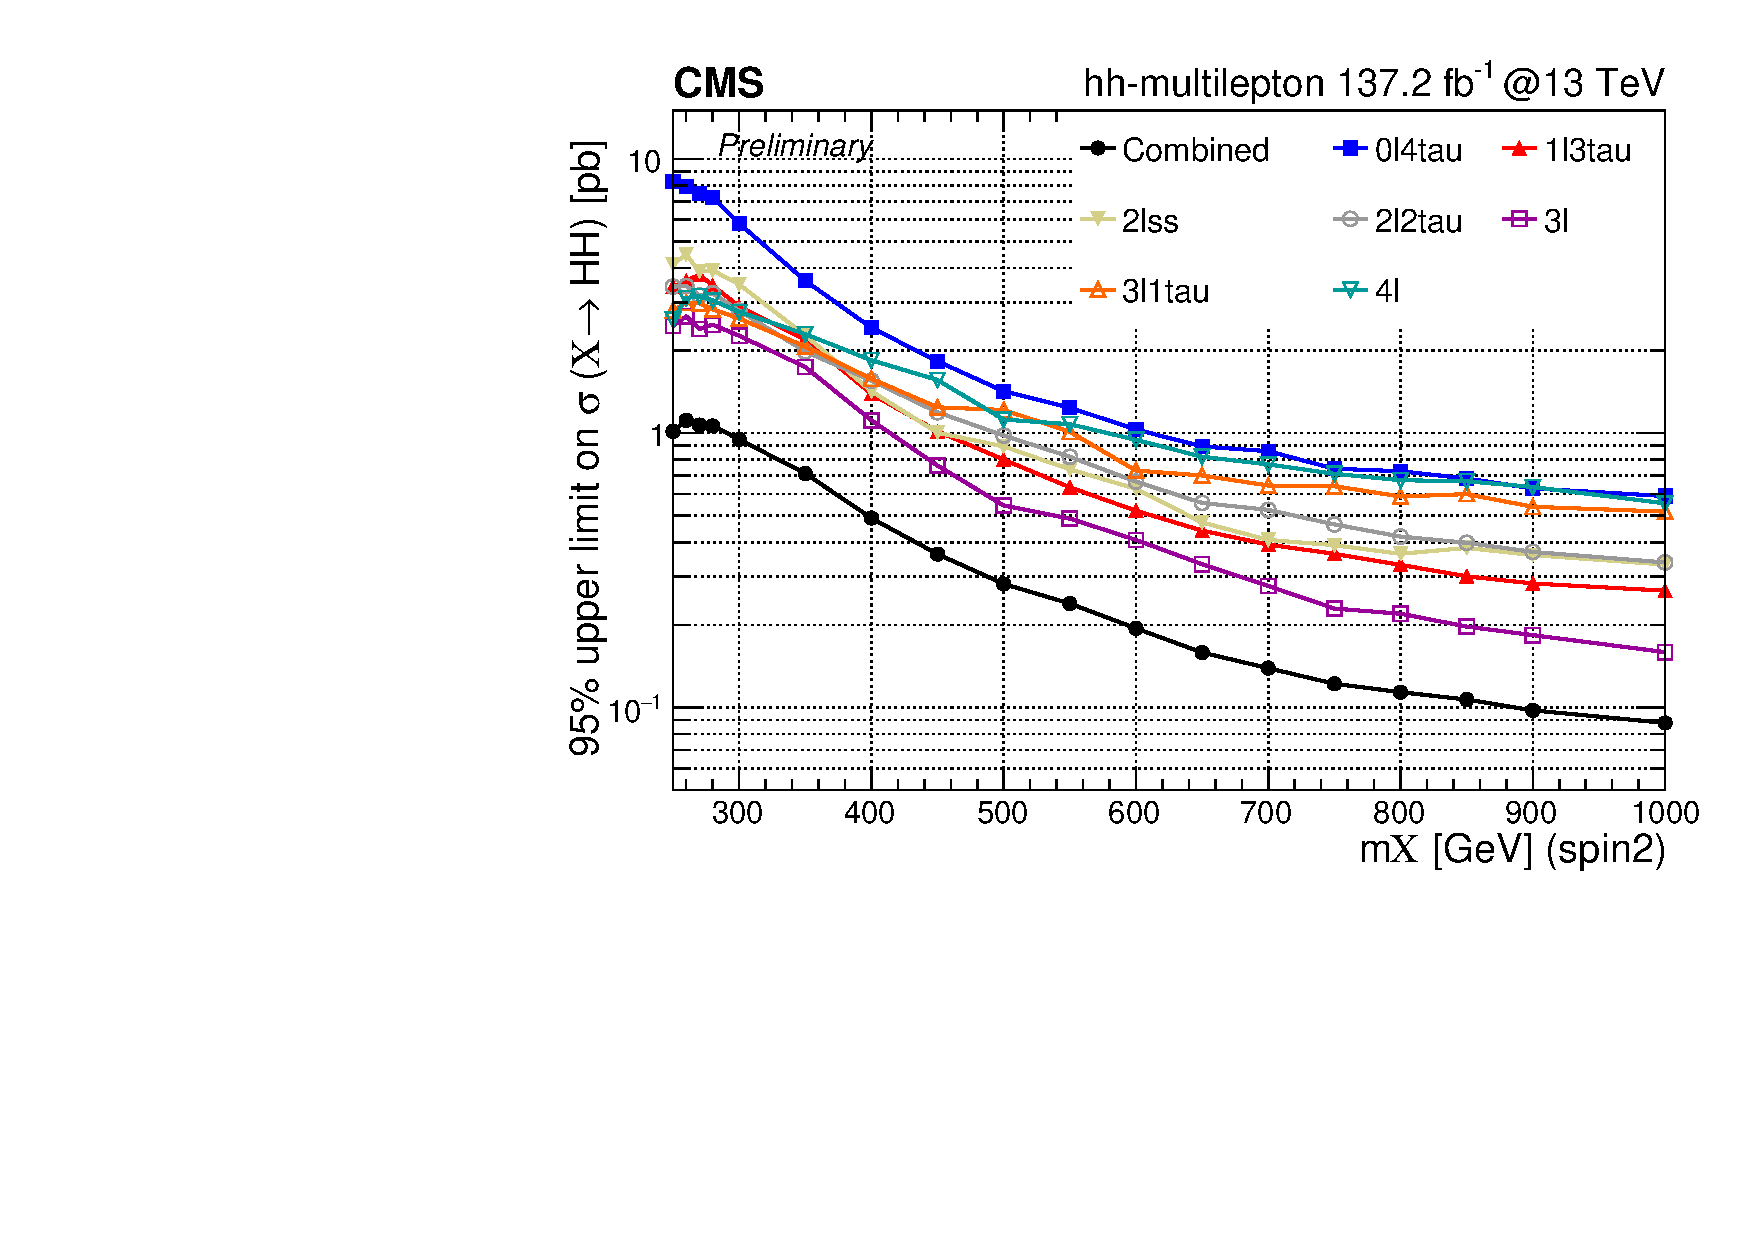
\includegraphics[width=0.45\textwidth]{figures/massMultiScan_spin2_multilepton_Run2.pdf}
  \caption{
    Observed and expected 95\% CL limits on the production of new particles $\X$ of spin $2$ 
    and mass $m_{\X}$ in the range $250 \leq m_{\X} \leq 1000\GeV$, which decay to $\PHiggs$ boson pairs,
    for the combination of all seven search categories (left)
    and for each search category separately (right).
  }
  \label{fig:HH_limits_spin2}
\end{figure}

\section{Summary}
\label{sec:summary}

The results of a search for non-resonant as well as resonant $\HH$ production in final states with electrons, muons, and $\tauh$ has been presented.
The search is based on proton-proton collision data recorded by the CMS experiment at $\sqrt{s} = 13\TeV$ center-of-mass energy,
corresponding to an integrated luminosity of $137.2\fbinv$,
and targets the $\HH$ decay modes $\PW\PW\PW\PW$, $\PW\PW\PGt\PGt$, and $\PGt\PGt\PGt\PGt$.
Seven distinct search categories, distinguished by the multiplicity of leptons and $\tauh$, are included in the analysis:
\llss, \lllnot, \llll, \lllt, \lltt, \lttt, and \noltttt.
No evidence for a signal is found in the data and upper limits on the cross section for non-resonant as well as resonant $\HH$ production are set.
The observed (expected) limits on non-resonant $\HH$ production range from $XX$ to $XX$ ($XX$ to $XX$)~\pb, depending on the coupling scenario.
For the case of non-resonant $\HH$ production with event kinematics equal to the kinematics expected in the SM,
the observed (expected) upper limit on the cross section amounts to $XX$ ($XX$) times the rate expected in the SM.
The results of the search for non-resonant $\HH$ production are used to exclude regions in the plane of the $\PHiggs$ boson coupling to the top quark, $\yt$,
and of the trilinear $\PHiggs$ boson self-coupling, $\lambda$.
Assuming $\yt$ has the value expected in the SM, the trilinear $\PHiggs$ boson self-coupling is constrained to be within the interval $X.X < \kappal < X.X$.
For resonant $\HH$ production, the observed (expected) limits on the $\HH$ production cross section range from $XX$ to $XX$ ($XX$ to $XX$)~\pb, 
depending on the mass of the resonance and on its spin.
All limits are quoted at $95\%$ CL.


\newpage

\bibliography{auto_generated}
